\chapter{\label{cha:pro_qua}Experiments on Varieties and Quality}
This chapter reports the results of experiments using linguistically-motivated translationese-aware features to distinguish experience-related varieties of translations and to estimate human translation quality on various types of human quality assessment. Importantly, these results are compared to the performance of several other representations to indicate the learnability of the available ontological labels and human judgment. 

%The results are reported in two groups of experiments run for the same types of document representations.

First, Sections~\ref{ssec:var} and~\ref{ssec:bin} have the results of binary classifications for student vs professional translations, and for documents with \textit{bad} and \textit{good} quality labels, which were obtained as described in Section~\ref{ssec:binary}. 
%In Section~\ref{ssec:pro} we argued that this ontological distinction might be relevant for quality. 
Second, Section~\ref{sec:_scores} explores the learnability of continuous quality scores generated (i) from  error annotation (as discussed in Section~\ref{ssec:err}) and (ii) from direct assessment (see Section~\ref{ssec:da}). The experiments on quality scores, formulated as regression tasks are extended to sentence level, because both types of assessment (unlike labels) were originally obtained for sentences and then averaged to get document scores. 
On the one hand, sentence-level tasks are expected to be more challenging for most of manual frequency-based features, but on the other hand they should be more natural for embeddings and less limiting in terms of the size of the training data. Additionally, scores from two different manual assessment methods (error annotation vs perceived quality) might offer dissimilar perspectives of translation quality.
Last, but not least, scores from error annotation allow to compare applicability of proposed representations for major theoretical quality aspects -- accuracy and fluency.

The classification tasks in Section~\ref{sec:labels} rely on the same experimental setup as described in Section~\ref{sec:my_classifiers} with regard to learning methods, alternative representation methods and feature analysis. However, we open this section with details on the datasets and on additional representation for varieties and quality classifications.
Additional specifics of regression experiments appear in the second part of the chapter, before we present the respective results (see Section~\ref{ssec:my_doc_regressors}).

\section{\label{sec:labels}Classification Tasks}

There are a few preliminary notes on the classification experiments reported in this section. 

\paragraph{Datasets} 
Classification experiments were run on the same dataset as translationese classifications. However, it does not mean that student translations were represented only by translations with either good or bad label. In fact, 334 student translations and 360 quality-labelled translations had only 25 instances in intersection (six labelled as \textit{good} and 19 as \textit{bad}). 

The binary labels used in this chapter are: 
\begin{description}\compresslist{}
	\item[stu vs pro:] categories in a classification to capture professionalism;
	\item[bad vs good:] categorial document-level quality labels from holistic assessment of student translations verified in a separate annotation effort (see Section~\ref{ssec:binary}).
\end{description}

\paragraph{QuEst++ baseline}
In addition to manual features investigated in this thesis, we implemented 61 of 78 available document-level QuEst++ features (\textit{quest61}) to ensure comparability of our results with previous research.
We had to exclude QuEst++ features which reflected the size of the documents -- number of tokens in the source document (\#1001), number of tokens in the target document (\#1002) and number of sentences in the target document (\#9801) because they would be a simple give-away for student and professional translations in our collections (see additional parameters of the respective document categories in Table~\ref{tab:corpus_means} on page~\pageref{tab:corpus_means}).  

\subsection{\label{ssec:var}Translation Varieties}

In this section we look at the differences between professional translation varieties when classified against each other. This opposition is interpreted as a proxy for quality on the assumption that student translations are inferior to professional due to the lack of experience (see Section~\ref{ssec:pro}). A useful reminder is that for this experiment the student translations were selected randomly from the available sets of multiple translations for each source text and they might come from various quality grades. 

The experiments in previous chapter demonstrated that students were not easier to tear apart from non-translations than professionals. In terms of returned F1-scores, the results for translationese classifications on professional translations were slightly higher than on student translations for representations that capture translation-related aspects of language, i.e. on manual feature sets and on sentence embeddings that were fine-tuned on translation quality (\textit{TQmono-m}). However, on \textit{tf-idf} and on vectors from generic word embedding models (\textit{ruRoberta} and \textit{mdeberta3}) the results for student translations were higher.

\paragraph{Experimental results}
Table~\ref{tab:stu-pro} has the results on classification of translation varieties. We explicitly added results on the content-dependent classifiers that were not shown before. These representations are described in \textit{Alternative document representations} in Section~\ref{sec:my_classifiers} on page~\pageref{pg:vectors}  and include vectors from \textit{tfidf, stsb-xlm-r-m, TQmono-m, ruRoberta} models.

\begin{table}[H]
	\centering
	\begin{tabular}{l|llll}
		\toprule
		rep   & Accuracy        & Precision       & Recall          & F1              \\
		\midrule
		chance          & 49.59 (+/-3.47) & 49.45 (+/-3.48) & 49.45 (+/-3.51) & 49.39 (+/-3.49) \\
		\midrule
		UD              & 76.55 (+/-5.15) & 77.05 (+/-5.39) & 76.32 (+/-4.77) & 76.24 (+/-5.01) \\
		collgram        & 65.02 (+/-5.29) & 65.50 (+/-6.24) & 63.70 (+/-5.27) & 63.25 (+/-5.74) \\
		ngram           & 66.80 (+/-5.64) & 67.11 (+/-6.12) & 66.32 (+/-5.60) & 66.07 (+/-5.74) \\
		all             & 79.67 (+/-3.50) & 79.85 (+/-3.48) & 79.46 (+/-3.32) & 79.43 (+/-3.46) \\
%		\midrule
		quest61         & 83.20 (+/-2.85) & 83.20 (+/-2.91) & 82.96 (+/-2.85) & \textbf{83.00} (+/-2.87) \\
%		quest17         & 77.78 (+/-4.71) & 77.92 (+/-4.85) & 77.76 (+/-4.96) & 77.57 (+/-4.80) \\
		\midrule
		tfidf           & 89.69 (+/-2.70) & 89.69 (+/-2.71) & 89.60 (+/-2.76) & \boxit{0.4in} 89.59 (+/-2.72) \\
		stsb-xlm-r-m          & 74.12 (+/-3.86) & 74.55 (+/-4.05) & 73.49 (+/-3.87) & 73.49 (+/-3.98) \\
		TQmono-m        & 84.28 (+/-3.70) & 84.87 (+/-3.45) & 83.68 (+/-3.98) & 83.89 (+/-3.89) \\
		ruRoberta & 87.26 (+/-4.22) & 87.73 (+/-4.40) & 86.95 (+/-4.25) & 87.05 (+/-4.29) \\
		mdeberta3  & 89.03 (+/-2.87) & 89.40 (+/-2.85) & 88.69 (+/-2.95) & 88.85 (+/-2.93)\\
		\bottomrule
	\end{tabular}
	\caption{\label{tab:stu-pro}Classification result for student vs professional labels by SVM. The highest F1-score for manual features is shown in bold, the highest result for content-dependent representations is boxed}
\end{table}

A glance at Table~\ref{tab:stu-pro} suggests that the best-performing representation on this task among manual features was the full QuEst++ feature set ($F1=83.28$). Among content-dependent classifiers, \textit{tf-idf} was not significantly outperformed by any other representation ($F1=89.59$). If we consider only statistically significant differences between representations for both SVM and neural classifier, we can observe the following. 

The relatively poor performance of translationese-aware UD feature sets against MT-quality-aware QuEst++ feature set (differences are statistically significant) suggest that the translationese-related distinctions between translation varieties were weaker than those captured by MT quality indicators (see feature analysis below).

Further on, \textit{tf-idf} was statistically superior to QuEst++. This means that the topical differences between the parallel corpora were even stronger than quality-related or translationese distinctions.

This line of interpretation is supported by the similarities in performance between QuEst++ and \textit{TQmono-m}, the two approaches designed to capture quality in MT, and between \textit{tf-idf} and \textit{mdeberta3}, which are thought to be focused on token-based properties (semantics) of documents. 

%The outcomes of significance testing between the representations is summarised in Table~\ref{tab:sign_tests_vars}. A hyphen indicates no differences, an asterisk stands for statistically significant differences as measured by t-test at the confidence level of 5\%.
%\todo[inline]{maybe delete these tables, or reorder them from by F1 res}
%\begin{table}[H]
%	\centering
%	\begin{tabular}{l|ccccccccc}
%		\toprule
%                		& UD  & collgr & ngram & all & quest61 & tfidf & stsb-xlm & TQmono & ruRoberta \\
%                \midrule
%		UD              &     &          &       &     &    &       &              &          & \\
%		collgram        & * * &          &       &     &    &       &              &         & \\
%		ngram           & * * & - -      &       &     &    &       &              &          & \\
%		all             & - - & * *      & * *   &     &    &       &              &         & \\
%		quest61         & * * & * *      & * *   & * - &    &       &              &          & \\
%		tfidf           & * - & * *      & * *   & * - & * * &       &              &       & \\
%		stsb-xlm        & - - & * *      & * *   & * - & * * & * -   &              &          & \\
%		TQmono          & * * & * *      & * *   & * - & - - & * -   & * *          &         & \\
%		ruRoberta       & * * & * *      & * *   & * * & * * & * *   & * *          & - *      & \\
%		mdeberta3       & * * & * *      & * *   & * * & * * & * *   & * *          & * *  & - - \\
%		\bottomrule
%	\end{tabular}
%	\caption{\label{tab:sign_tests_vars}Professionalism: Results on pair-wise significance testing on SVM (left marker) and neural classifier (right marker)}
%\end{table}

To further explore the success of QuEst++ features, RFECV was run on this feature set and the 25 selected features were analysed. This selection improved the performance of the classifier by 3\% against the entire feature set in terms of F1-score (86.17\% vs 83.00\%, the difference was statistically significant). 

We noticed that 15 of 25 features selected by the algorithm described the SL side (complexity features), seven features reflected target properties (fluency features), and 3 features were ratios of the two (adequacy features). 
The five most prominent ST-related QuEst++ features included \textit{percentage of punctuation marks in the source} (\#1074), \textit{source sentence perplexity without end of sentence marker} (\#1011), lemma repetition in the source document (\#9991), average number of translations per source word in the document (\#1024) and average source token length (\#1006).
% It can be seen that these features highlight the differences between the source texts in the two parallel subcorpora, implicitly introducing another reference corpus -- newspaper texts from the BNC -- into the comparison (see source sentence perplexity features). It looks like English texts translated by students were less familiar to the trigram LM learnt on the BNC.
Given that the sources of student and professional translations were different, it was not surprising that QuEst++ feature set worked well. However, it is difficult to interpret the  distinctions revealed between student and professional translations by this feature set as related to professionalism or quality. For this feature set, which explicitly uses ST complexity features, either the input to the translation process or the method of translation (type of human subjects, in our case) need to be the same.

The prominent fluency and adequacy features that can be viewed as relatively independent of the properties of ST and can be interpreted as related to quality in our experimental setup. Selected \textit{fluency features} were \textit{number of occurrences of the target word within the target hypothesis or TTR} (\# 1015), \textit{log probability of the target} (\# 1012), \textit{perplexity of the target document without end of sentence markers} (\# 1014). 
The log probabilities of student translations were on average lower than for professional translations and perplexity scores were higher for students. We can hypothesize that student translations were more surprising than professionals for the Russian LM trained on a comparable corpus. This confirms our findings in Section~\ref{ssec:best_ngram} (page~\pageref{pg:stu_more_surprising_than_pro}) and can be indicative of the presence of `strange strings' and awkward word choice, a common problem in student translations, accounting for up to 30\% of all annotated errors (see Figure~\ref{fig:errors500stacked}, page~\pageref{fig:errors500stacked}).
As expected, TTR was lower for student translations. It is a well-known translationese indicator: translations tend to have lower TTR than non-translations. % But this feature can also be interpreted as reflecting the differences in the source text register.
% The absolute values for the negative log probability calculated by QuEST++ 

\label{pg:quest_adequacy_feats_for_vars}
The \textit{adequacy features} selected by RFECV included only three features: \textit{ratio of number of tokens in source and target} (\#1003), \textit{ratio of number of tokens in target and source} (\#1004) and \textit{ratio noun repetition between target and source documents} (\#9996). The comparison of average values for professional and student translations showed that professional translations were more wordy but less repetitive. 

Despite QuEst++ feature set was not entirely fit for our purposes, the relevant parts of it confirmed that \textbf{student translations were indeed different from professional translations in terms of quality-related features of fluency and adequacy}.

%The features from this selection that also had significant differences between two categories and big LogR F1-score in a single-feature setup are described in Table~\ref{tab:best_quest}.
% I need features selected by RFECV with sorted by LogR F1-score with means (no comparison to ref possible)
%\begin{table}[H]
%	\centering
%	\begin{tabular}{l|p{8cm}cll}
%		\toprule
%		ID   & description & SVM weight       & LogR          & means    \\
%		\midrule
%		1074 & percentage of punctuation marks in source & -1.824 & 0.58 & stu<pro \\
%		1075 & percentage of punctuation marks in target & 2.037 & 0.57 & stu<pro \\
%		1015 & number of occurrences of the target word within the target hypothesis (averaged for all words in the hypothesis, TTR) & -1.800 & 0.45 & stu<pro \\
%		1012 & log probability of the target & 0.971 & 0.40 & stu<pro \\  % negative
%		1011 & source sentence perplexity without end of sentence marker & 0.607 & 0.35 & stu>pro \\ % stu: three times higher
%		1010 & source sentence perplexity & 1.378 & 0.30 & stu>pro \\ % twice higher
%		\bottomrule
%	\end{tabular}
%	\caption{\label{tab:best_quest}Student vs professional translations: best QuEst++ features}
%\end{table}

%\begin{table}[H]
%	\centering
%	\begin{tabular}{l|lll|p{8cm}}
%		\toprule
%		 & LogR & means & SWM weight & description \\
%		1074 & 0.58 +/-0.06 & stu\textless{}pro & -1.867 & percentage of punctuation marks in source \\
%		1075 & 0.57 +/-0.07 & stu\textless{}pro & 2.105 & percentage of punctuation marks in target \\
%		1015 & 0.45 +/-0.07 & stu\textless{}pro & -1.709 & number of occurrences of the target word within the target hypothesis \\
%		1012 & 0.40 +/-0.10 & stu\textgreater{}pro & 0.993 & log probability of the target \\
%		1011 & 0.35 +/-0.05 & stu\textgreater{}pro & 0.411 & source sentence perplexity without end of sentence marker \\
%		9991 & 0.31 +/-0.12 & stu\textless{}pro & -0.529 & Lemma repetition source document \\
%		1010 & 0.30 +/-0.05 & stu\textgreater{}pro & 1.425 & source sentence perplexity \\
%		1003 & 0.24 +/-0.10 & stu\textgreater{}pro & 0.675 & ratio of number of tokens in source and target \\
%		1004 & 0.23 +/-0.10 & stu\textless{}pro & 0.728 & no tokens in the target / no tokens in the source \\
%		1024 & 0.20 +/-0.07 & stu\textgreater{}pro & 0.663 & average number of translations per source word in the document (threshold in giza1: prob \textgreater 0.5) \\
%		1006 & 0.20 +/-0.06 & stu\textgreater{}pro & -0.251 & average source token length \\
%		9995 & 0.16 +/-0.12 & stu\textless{}pro & 0.626 & noun repetition in source document \\
%		1013 & 0.16 +/-0.05 & stu\textgreater{}pro & 0.378 & perplexity of the target document \\
%		9989 & 0.02 +/-0.04 & stu\textless{}pro & 2.090 & Lemma repetition target \\
%		9994 & 0.02 +/-0.04 & stu\textless{}pro & -0.886422499648305 & Noun repetition in target document \\
%		1036 & 0.00 +/-0.00 & stu\textless{}pro & -0.768113106194483 & average number of translations per source word in the document (threshold in giza: prob \textgreater 0.01) weighted by the inverse frequency of each word in the source corpus \\
%		1058 & 0.00 +/-0.00 & stu\textgreater{}pro & 0.436312660340393 & percentage of distinct unigrams seen in the corpus (in all quartiles) - document-level \\
%		1014 & 0.00 +/-0.00 & stu\textgreater{}pro & 0.530362133473979 & perplexity of the target document without end of sentence markers \\
%		1034 & 0.00 +/-0.00 & stu\textgreater{}pro & 1.2297283646799 & average number of translations per source word in the document (threshold in giza1: prob \textgreater 0.5) weighted by the frequency of each word in the source corpus \\
%		1044 & 0.00 +/-0.00 & stu\textless{}pro & -0.120421040410991 & average number of translations per source word in the document (threshold in giza: prob \textgreater 0.5) weighted by the inverse frequency of each word in the source corpus \\
%		1061 & 0.00 +/-0.00 & stu\textgreater{}pro & -0.627253206323009 & average word frequency: on average, each type (unigram) in the source document appears x times in the corpus (in all quartiles) \\
%		1046 & -- & stu\textgreater{}pro & 0.184878659979718 & average unigram frequency in quartile\_1 of frequency (lower frequency words) in the corpus of the source document") \\
%		1028 & -- & stu\textless{}pro & 0.779970315329144 & average number of translations per source word in the document (threshold in giza1: prob \textgreater 0.5) weighted by the frequency of each word in the source corpus \\
%		1059 & -- & stu\textless{}pro & -0.882345735462283 & percentage of distinct bigrams seen in the corpus (in all quartiles) - document-level \\
%		9996 & -- & stu\textgreater{}pro & 0.354557501871447 & Ratio noun repetition between target and source docuemnts\\ 
%		\bottomrule
%	\end{tabular}
%\caption{\label{tab:best_quest}Student vs professional translations: best QuEst++ features}
%\end{table}

%1003 ratio of number of tokens in source and target (stu: higher, logreg: 0.24) 1.10 +/-0.16,1.05 +/-0.08
%1004 no tokens in the target / no tokens in the source (stu: smaller, logreg: 0.23) 0.93 +/-0.12,0.96 +/-0.08

 
% the negative of the average log probability is the information entropy of an event
% Since the probabilities of independent events multiply, and logarithms convert multiplication to addition, log probabilities of independent events add.
%  log probabilities can only represent non-zero probabilities. Since the logarithm of a number in {\displaystyle (0,1)}(0,1) interval is negative, often the negative log probabilities are used.


%The lack of punctuation marks in students subcorpus might reflect difference in the corpora content rather than true translation-related phenomena. We believe it is the lack of (heavily punctuated) direct speech in the full size newspaper reportage but limited in translations of the a few opening paragraphs of otherwise similar documents, a typical task in a translation class.

%Best features (15): ['adp', 'cconj', 'content\_TTR', 'copula', 'neg', 'nn', 'sconj', 'acl:relcl', 'appos', 'case', 'conj', 'ccomp', 'iobj', 'mark', 'parataxis']
Turning to the analysis of best performing UD feature, we can report that a classifier limited to 15 RFECV-selected features improved the performance on this task by three percentage points from F1-score 76.24\% to 79.39\%. % the difference was still NOT significant!
Only six of these 15 strong predictors of professional varieties in translations were also among strong translationese indicators\wlvfootnote{The lists of UD features include the shorthand names used for albathetised description in Appendix~\ref{appx:ud}}. This list included frequencies of \textit{relative clauses (acl:relcl)}, \textit{clausal complements (ccomp)}, \textit{copula verbs (copula)}, \textit{negative particles (neg)}, \textit{function words indicating the head of a subordinate clause (mark)}, \textit{subordinating conjunctions (sconj)}.

Other six features come from the subsets of translationese indicators that were specific only to professional (\textit{prepositions (adp)} , \textit{function of analytical case markers (case)}, \textit{type-to-token ratio (content\_TTR)} ) or student translations (\textit{asyndetically introduced elements (parataxis)}, \textit{indirect objects (iobj)}, \textit{nouns (nn)}).

The third subset (\textit{appositional modifiers of nouns (appos)}, \textit{coordinating conjunctions (cconj)}, \textit{syntactic conjuncts (conj)}) included features that were not selected in either of the translationese classifications.

Based on the performance of single-feature classifier (if there were statistical distinctions between the categories in the first place), these features cannot be viewed as capturing large distributional dissimilarities between student and professional translations. 
Only seven out of 15 selected features had statistically different values between the categories. The highest association score among them was observed for \textit{parataxis}: LogReg F1-score for this feature was estimated at a modest level of 34\%. 

It was shown in the previous chapter that both translation varieties deviated from the expected TL norm along the same dimensions suggestive of similar patterns in translational behaviour. 
Despite professionalism was captured fairly well by UD features (F1 = 79.39\% on the best-performing subset), the differences between the varieties can hardly be explained by translationese.
\label{pg:more_professional_more_translated} If anything, some expected translationese trends were better expressed in professional translations (based on the features with statistical differences): professional translators used more markers of dependent clauses, clausal complements, epistemic markers, modal predicates as well as fewer nouns. % (0.27 vs 0.24)
In English-to-Russian translation these features might indicate carrying over the English patterns rather than adopting to the TL norm. % given the
Some strong translationese predictors (\textit{acl:relcl, copula, determiners, finite verbs}) did not have statistical differences between the categories.
On the other hand, professional translations had more varied vocabulary evidenced by higher TTR, more indirect objects and negative particles, fewer analytical passives. These properties are indicative of stronger normalisation trends along these dimensions.

\subsection{\label{ssec:bin}Binary Quality}
This section presents the results of the same analytical procedure applied to document-level quality labels. 
Our major question is whether the identified translationese indicators consistently contribute to predicting `good' and `bad' translation. 

The dataset with binary quality labels is summarised in Table~\ref{tab:binqua_pars}. It can be seen that the categories are reasonably balanced, with a bit fewer good translations. Recall from Section~\ref{sec:mygold} that these documents come from sets of multiple student translations for 57 English mass-media source texts, and include from one to four translations in each quality category for each ST.

\begin{table}[]
	\centering
	\begin{tabular}{l|c|c|cc|cc}
		\toprule
		% for simplicity I averaged the diverging number of sentences between src and tgt. This divergence is due to independent sentence-splitting and filtering out shards of sentences after lemmatisation
		       & documents & sentences & \multicolumn{2}{c|}{tokens} & \multicolumn{2}{c}{tokens per doc} \\
		       &           &           & EN      &  RU              & EN      &  RU \\
		\midrule  
		bad     & 183  	   & 4 144    & 93,844 & 87,894           & 512.81 (+/-117.39) & 480.30 (+/-114.76) \\  
		good    & 177      & 4 070    & 89,536 & 85,560           & 505.85 (+/-108.44) & 483.39 (+/-111.83) \\ 
		\bottomrule
	\end{tabular}
	\caption{\label{tab:binqua_pars} Basic parameters of parallel subcorpus with binary quality labels (after preprocessing and lemmatisation)}
\end{table}
%                bad 183
%good 177
%Length of labels array: 360
%Shape of mdeberta3 reps: (360, 768)

Table~\ref{tab:bad-good} reports SVM outcomes for 10 representation of student translations labelled for binary quality. The results for the neural classifier appear in Appendix~\ref{appx:neural_res} (see Table~\ref{tab:stu-pro_neu}). As before, below the performance of various representations is compared based on the agreed outcomes of SVM and neural model.
Out of 10 representations attempted, statistically significant differences between SVM and neural classifier were seen only on \textit{stsb-xlm-r-m} vectors, where SVM outperformed the neural model. 

\begin{table}[H]
	\centering
	\begin{tabular}{l|llll}
		\toprule
		rep      & Accuracy         & Precision        & Recall           & F1               \\
		\midrule
		chance          & 51.67 (+/-7.78) & 51.67 (+/-7.80) & 51.67 (+/-7.78) & 51.63 (+/-7.78) \\
		\midrule
		UD              & 61.39 (+/-5.75) & 61.60 (+/-5.81) & 61.29 (+/-5.82) & 61.00 (+/-5.93) \\
		collgram        & 57.78 (+/-9.53) & 58.04 (+/-9.99) & 57.87 (+/-9.73) & 57.36 (+/-9.81) \\
		ngram           & 47.22 (+/-4.48) & 47.29 (+/-4.53) & 47.42 (+/-4.41) & 46.73 (+/-4.51) \\
		all             & 62.50 (+/-7.68) & 62.70 (+/-7.92) & 62.45 (+/-7.76) & \textbf{61.99} (+/-8.21) \\
%		\midrule
		quest61         & 47.22 (+/-6.92) & 47.23 (+/-6.96) & 47.28 (+/-6.91) & 46.96 (+/-6.92) \\
%		quest17         & 51.94 (+/-7.66) & 51.84 (+/-8.05) & 51.82 (+/-7.81) & 51.56 (+/-7.87) \\
		\midrule
		tfidf           & 59.17 (+/-6.34) & 59.19 (+/-6.51) & 59.11 (+/-6.47) & 58.92 (+/-6.58) \\
		stsb-xlm-r-m          & 61.67 (+/-9.92) & 61.70 (+/-9.94) & 61.66 (+/-9.93) & 61.61 (+/-9.93) \\
		TQmono-m        & 63.06 (+/-6.22) & 63.42 (+/-6.10) & 63.11 (+/-6.01) & 62.77 (+/-6.34) \\
		ruRoberta & 75.00 (+/-7.14) & 75.50 (+/-7.42) & 75.02 (+/-7.14) & 74.89 (+/-7.13) \\
		mdeberta3  & 78.33 (+/-6.89) & 78.88 (+/-6.48) & 78.34 (+/-6.93) & \boxit{0.4in}78.14 (+/-7.13)\\
		\bottomrule
	\end{tabular}
	\caption{\label{tab:bad-good}Binary quality classification results by SVM. The highest F1-score for manual features is shown in bold, the highest result for content-dependent representations is boxed}
\end{table}
In this classification, UD performed significantly better than all other hand-engineered features, including features from QuEst++ framework. The concatenation of UD with collgram- and unigram-based features did not yield a significant increase in performance. 

This task proved much more challenging for content-dependent classifiers than translation detection task or classification of professional varieties. It is not surprising as the classifiers were faced with a content-wise much more homogeneous set of documents, in fact, with multiple translations of the same source text. There were no statistically significant differences between the performance of UD features and \textit{tf-idf} or vectors from two sentence embedding models (\textit{stsb-xlm-r-m} and \textit{TQmono-m}).
However, representations produced as triple aggregation of word vectors using \textit{ruRoberta} and \textit{mdeberta3} models, remained unbeaten in absolute terms, with no difference between them, as was the case with all other classifications. 
%The results of statistical significance tests between representations are presented in Table~\ref{tab:sign_tests_qua_labels}. In each pair of markers in the table, the first one is for SVM and the second -- for the neural classifier; asterisk indicates statistical significance of observed differences.
%\todo[inline]{lose these tables}
%\begin{table}[H]
%	\centering
%	\begin{tabular}{l|ccccccccc}
%		\toprule
%		& UD  & collgr & ngr & all & quest61  & tfidf & stsb-xlm & TQm & ruR \\
%		\midrule
%		UD              &     &      &    &         &         &       &  &   & \\
%		collgram        & - - &      &    &         &         &       &  &  & \\
%		ngram           & * - & * -  &    &         &         &       &   &    & \\
%		all             & - - & - -  & * - &        &         &       &    & & \\
%		quest61         & * * & * -  & - - & * *    &         &       &  & &  \\
%		tfidf           & - - & - -  & * - & - -    & * *     &       &    &  &  \\
%		stsb-xlm        & - - & - -  & * - & - -    & * -     & - -   &      &    &    \\
%		TQmono          & - - & - *  & * * & - -    & * *     & - *   & - *  &      & \\
%		ruRoberta       & * * & * *  & * * & * *    & * *     & * *   & * *  & * *  &   \\
%		mdeberta3       & * * & * *  & * * & * *    & * *     & * *   & * *  & * *  & - - \\           
%		\bottomrule
%	\end{tabular}
%	\caption{\label{tab:sign_tests_qua_labels}Quality labels: Results on pair-wise significance testing on SVM (left marker) and neural classifier (right marker)}
%\end{table}
Hand-crafted UD features designed to capture translationese (and successful in that task as was shown in Chapter~\ref{cha:translationese}) were secondary only to the recent large pre-trained word embeddings in the current task of document-level human translation quality estimation. UD features achieved $F1=61.00$\wlvfootnote{Note that feature selection improved this result to reach $F1=68.9$, see page~\pageref{pg:selection_helps_in_quality_classification}} vs $F1=78.14$ on \textit{mdeberta3} vectors.
Admittedly, their performance was very limited in the proposed binary classification setup. It was still above the random baseline, which was not the case for alternative representations. 

Good performance of embedding models is reassuring, because it means that the quality distinctions annotated in our dataset were actually related to objective properties of the texts, and not as subjective as it was commonly believed with regard to human annotation of quality at document level. 
Although we cannot be entirely sure which linguistic properties of translations were captured by the best performing \textit{mdeberta3} vectors, the lack of topical variation between good and bad translations in this experimental setup, allows a cautious conclusion that the vectors actually reflected quality-related aspects of language. 
% These aspects may or may not be aligned with translationese properties of the documents.  % Aspects of quality manifested in the TT only and not translationese? 

The panels in Figure~\ref{fig:pca_qua} reflect the differences between quality categories as captured by the full UD feature set and \textit{mdeberta3} model. UD features clearly put student translations in the gap between source and target languages, with top-ranking translations being a bit shifted towards the non-translated TL side of the continuum. 
Vectors from \textit{mdeberta3}, a multilingual model, primarily capture the language distinction at D1. This squeezes the Russian language varieties into the same location on the plot and overshadows the differences between them. Nonetheless, top-ranking translations are clearly further away from sources, than low-ranking translations. This might mean that top-ranking translations are more distant from their sources and more adopted to the TL norm. 
\begin{figure}[H]
	\begin{minipage}[c]{0.5\linewidth}
		\centering
		UD features PCA D1
		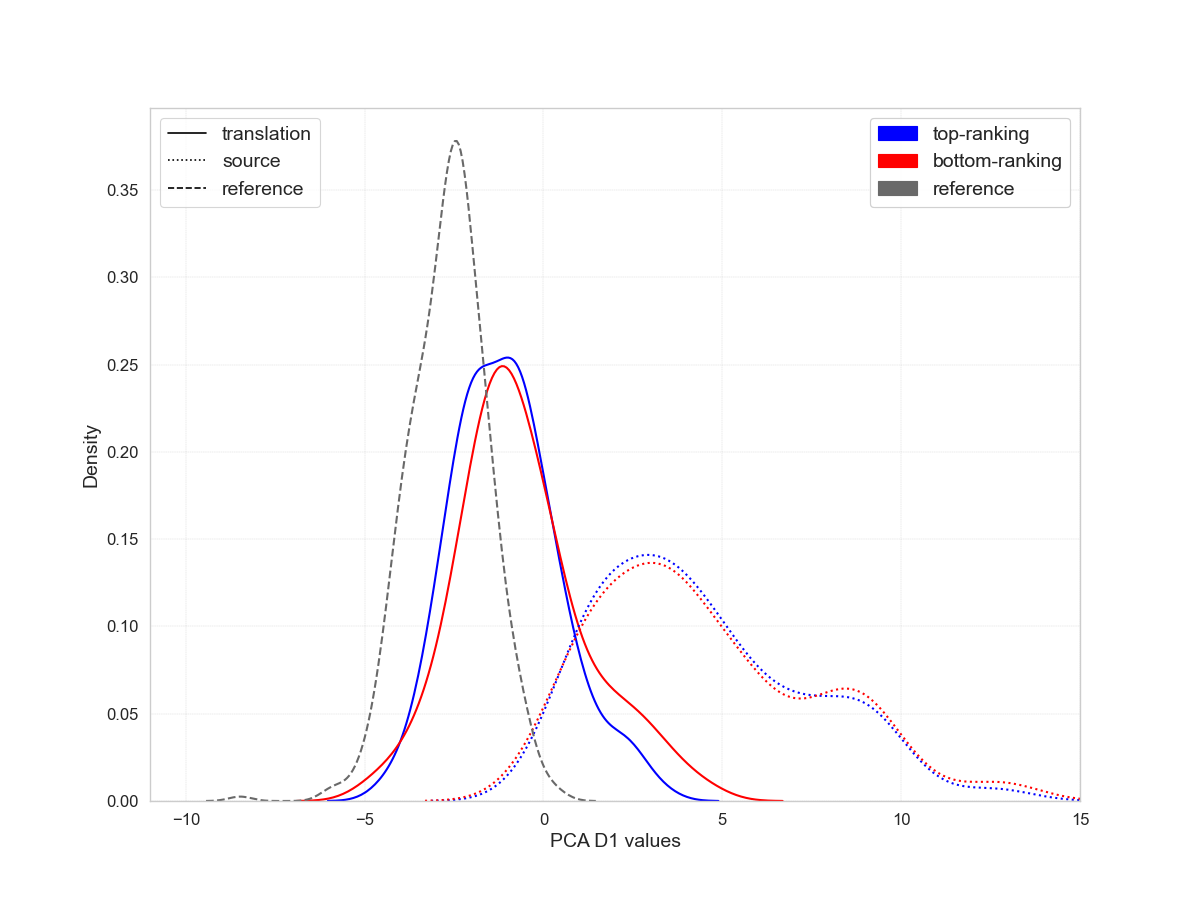
\includegraphics[width=\linewidth]{figures/pca/src-qua-ttype-ud-PCA-D1-lines}
	\end{minipage}	
	\begin{minipage}[c]{0.5\linewidth}
		\centering
		\textit{mdeberta3} PCA D1
		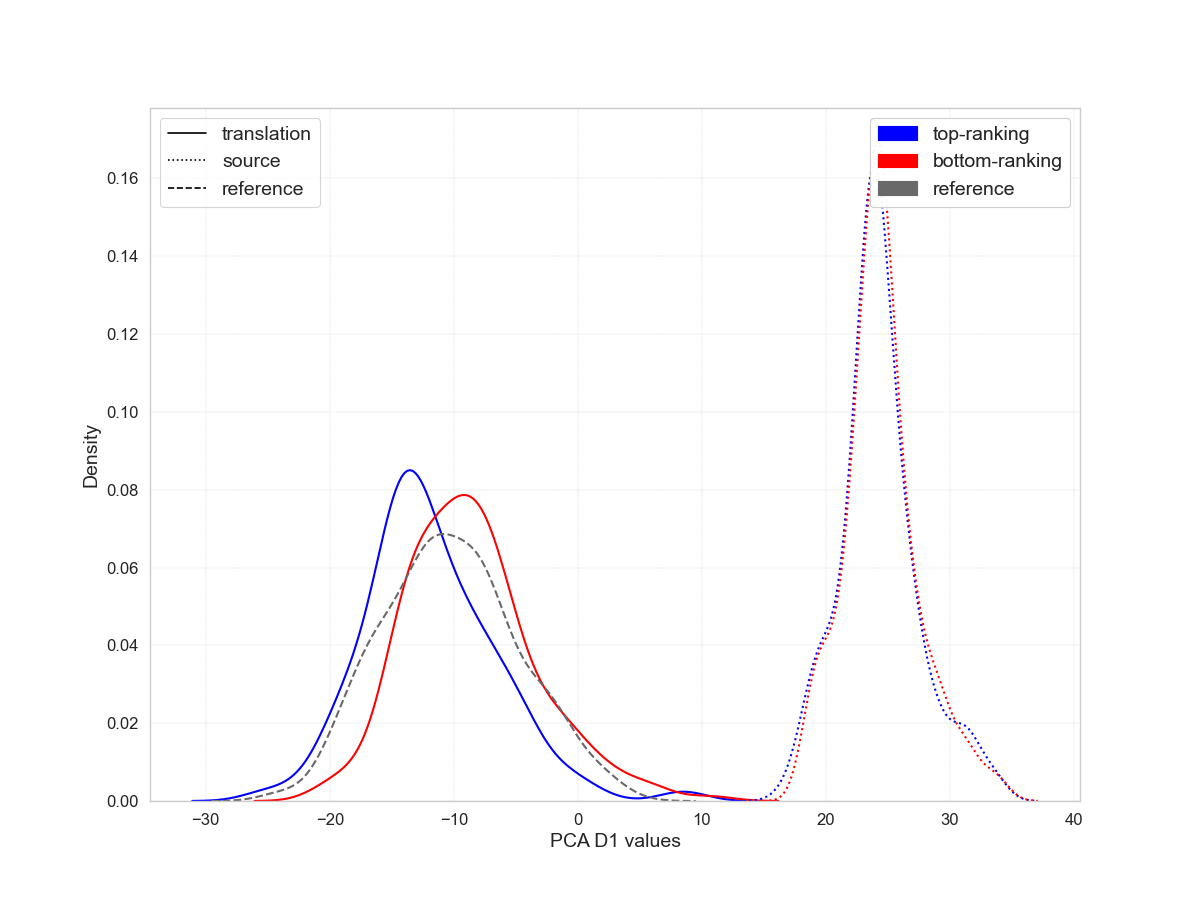
\includegraphics[width=\linewidth]{figures/pca/src-qua-ttype-mdeberta3-base-PCA-D1-lines}
	\end{minipage}
	\caption{\label{fig:pca_qua}Variability of PCA D1 values in quality-annotated documents (along with their sources and non-translations)}	
\end{figure}   

In turn, this suggests that the quality distinctions captured by \textit{mdeberta3} are, in fact, related to translationese, interpreted as the amount of deviations from the TL norm, especially on the axis capturing language contrast.
\begin{figure}[H]
	\begin{minipage}[c]{0.5\linewidth}
		\centering
		Top 26 UD features PCA D1
		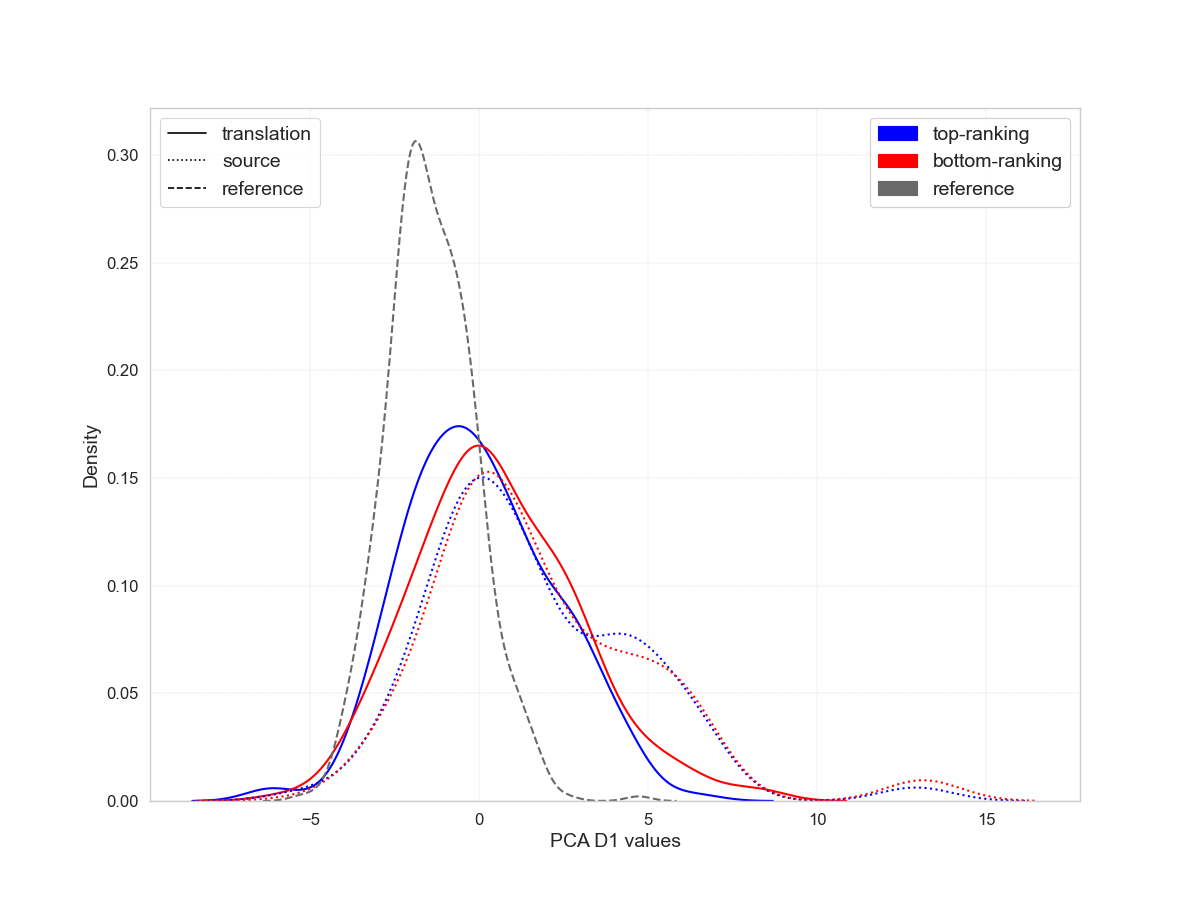
\includegraphics[width=\linewidth]{figures/pca/src-bad-good-pca-ud26-D1-lines}
	\end{minipage}	
	\begin{minipage}[c]{0.5\linewidth}
		\centering
		\textit{mdeberta3} PCA
		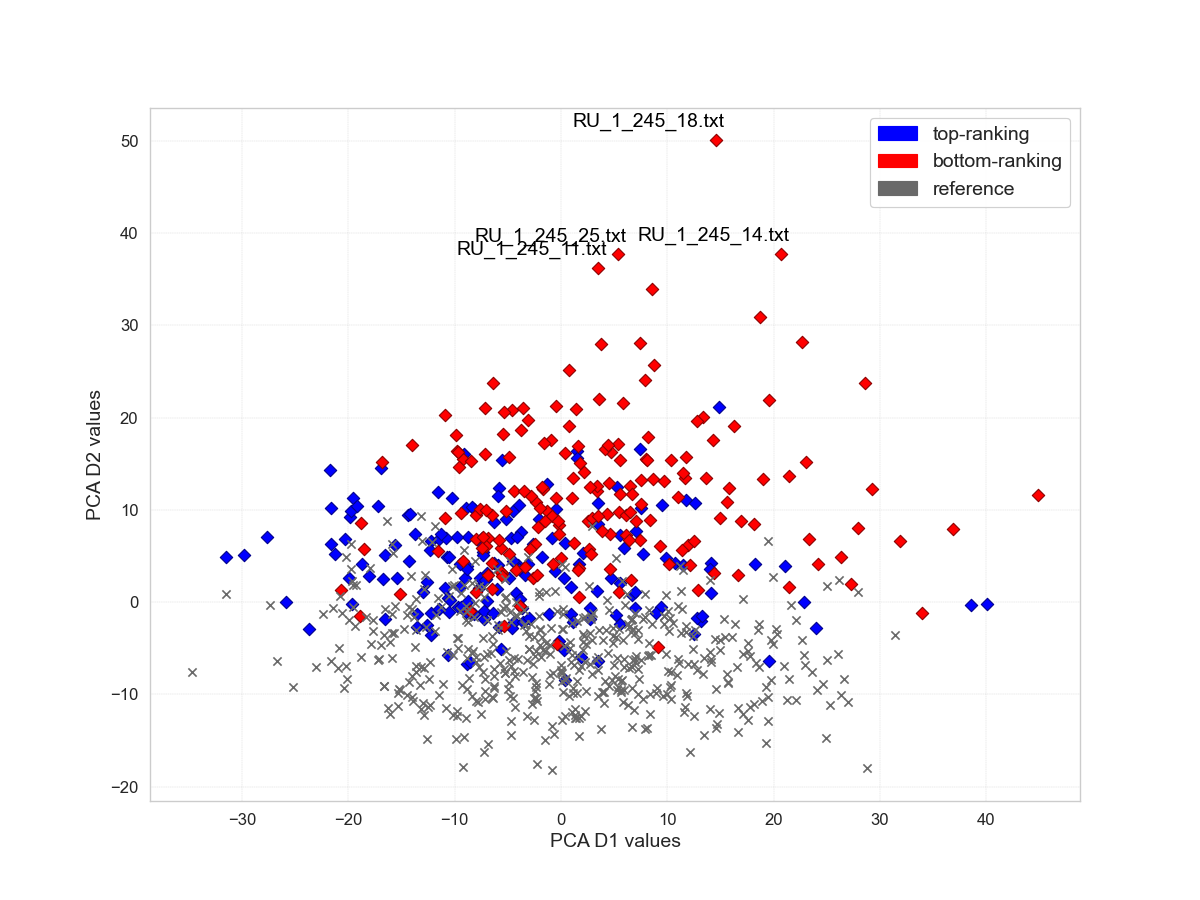
\includegraphics[width=\linewidth]{figures/pca/qua-ttype-mdeberta3-base-PCA-scatter}
	\end{minipage}
	\caption{\label{fig:pca_qua26}Variability of PCA D1 values in quality-annotated documents (no source texts)}	
\end{figure}
However, as we have seen in the feature analysis for student translations in Section~\ref{ssec:best_ud}, shining-through does not exhaust translationese manifestations. Plotting the PCA results for just the best performing subset of UD features eliminated the distinctions between languages (compare the left-hand panels in Figures~\ref{fig:pca_qua} and~\ref{fig:pca_qua26}). This might mean that some of the 26 selected features (see below) are not necessarily shining-through indicators. Translation quality is partly captured along other dimensions of translated language, not just the one defined by the contrast between languages. 

The right-hand panel in Figure~\ref{fig:pca_qua26} demonstrates that the PCA transform of the \textit{mdeberta3} captures the quality parameter of the dataset on the orthogonal PCA dimension (D2): the lower-ranking translations (in red) can be identified as more distant from TL norm (grey cloud). 
% RU_1_245_25.txt
%RU_1_245_11.txt
%RU_1_245_18.txt
%RU_1_245_14.txt

\paragraph{\label{pg:selection_helps_in_quality_classification}Feature analysis} 
Almost half of 26 most contributing UD features selected by RFECV in the classification task on quality labels were in the intersection with strong translationese indicators identified in Section~\ref{ssec:best_ud}. This selection significantly improved the performance of the SVM classifier: F1-score went up by 8\% from 61.0 to 68.9\%. 
%68.86 (+/-7.15)
%T-TEST: svm_bad-good_ud26 is significantly better with F1-score = 0.6886167230000001

Table~\ref{tab:bad-good_indicators} aggregates parameters that characterise each feature in this selection from the point of view of: (1) ability to predict quality categories alone (for features with statistically significant differences between the categories, otherwise `--' in \textit{LogR} column), (2) comparison of mean feature values across the categories, (3) SVM weights assigned to each feature and (4) translational trend in `bad' translations. 
The hypothesised trend is shown in bold if there were significant differences between `good' and `bad' categories. The regular font is used if there were significant differences between some of the three document categories involved in the comparison (src, bad, ref). In cases where there were no distinctions between the three categories, it was difficult to talk about any trend (--). The table is sorted by SVM weight.
% for intersection with pro, it is everything except case
% for intersection with student: not used for qua 7 of 14: 'aux', 'superl', 'xcomp', 'infs', 'mhd', 'nn', 'content_dens'

%Best Feats within levels with skewed distributions (4): ['good_adp', 'bad_adp', 'bad_mdd', 'bad_simple']
%Best Feats with unequal variances (22): ['adp', 'attrib', 'caus', 'content_TTR', 'deverbals', 'mdd', 'mpred', 'mquantif', 'numcls', 'possp', 'pverbals', 'sentlength', 'simple', 'advcl', 'amod', 'appos', 'aux:pass', 'conj', 'iobj', 'nummod', 'obj', 'parataxis']

%Strong translationese indicators useful for quality classification (12):{'advcl', 'attrib', 'acl:relcl', 'nsubj', 'pverbals', 'aux:pass', 'mark', 'obj', 'sentlength', 'amod', 'simple', 'deverbals'}

% it would be useful to add ref and type of trend to this table!!!
\begin{longtable}{l|llcc}
%	\centering
%	\begin{tabular}
		\midrule
		feature      & LogR         & means            & SVM weight &  trend in `bad' \\
		\midrule
		\textbf{sentlength}   & --           & bad=>good & 1.616 & NA  \\
		\textbf{nsubj}        & 0.13 +/-0.12 & bad>src>good>ref & 1.06  & \textbf{anglicisation} \\
		\textbf{amod}         & --           & bad=>good=>ref>src & 0.857 & adaptation \\
		\textcolor{Dandelion}{numcls}       & -- & bad>good>src=>ref & 0.713 & SL/TL indep \\
		\textbf{attrib}       & --           & bad=>good=>ref>src & 0.623 & adaptation \\
		\textbf{acl:relcl}    & 0.13 +/-0.09 & src>bad>good>ref & 0.615 & \textbf{shining} \\
		\textbf{simple}       & --           & src>ref=>bad=>good* & 0.563 & adaptation \\
		\textbf{advcl}        & 0.13 +/-0.07 & src>bad>good>ref & 0.521 & \textbf{shining} \\
		\textbf{aux:pass}     & --           & src>bad=>ref=>good & 0.491 & adaptation \\
		\textbf{deverbals}    & --           & bad=>good=>ref>src & 0.477 & adaptation \\
		\textbf{obj}          & --           & src>bad=>good>ref & 0.44  & shining \\
		\textcolor{cadmiumgreen}{content\_TTR} & 0.00 +/-0.00 & bad<good<=src<=ref & 0.416 & \textbf{SL/TL indep} \\
		\textbf{mark}         & --           & src>bad=>good>ref & 0.409 & shining \\
		\textcolor{Dandelion}{parataxis}    & --  & src<bad<=good<ref    & 0.397 & underuse of TL \\
		conj         & --           & bad=>good>src=>ref & 0.389 &  SL/TL indep \\
		\textcolor{cadmiumgreen}{passives}     & 0.05 +/-0.08 & src<bad<good<ref & 0.32 & \textbf{underuse of TL} \\
		\textcolor{Dandelion}{iobj}    & 0.05 +/-0.13 & src<bad<good<ref & 0.319 & \textbf{underuse of TL} \\
		\textcolor{Dandelion}{nummod}  & -- & ref=>bad=>good>=src* & 0.318 & -- \\
		\textcolor{cadmiumgreen}{mdd}  & -- & ref<bad<=good<src*    & 0.316 & normalisation \\
		\textbf{pverbals}     & --     & ref>bad=>good>src* & 0.289 & normalisation  \\
		\textcolor{cadmiumgreen}{adp}  & -- & src=>ref=>bad=>good & 0.254 & -- \\
		\textcolor{Dandelion}{mquantif}& -- & bad<=good<=ref<src & 0.244 & underuse of TL  \\
		appos        & --           & bad=>good=>ref=>src & 0.23 & --  \\
		possp        & --           & src<ref<=bad<=good*    & 0.202 & adaptation \\
		\textcolor{Dandelion}{caus} & -- & ref<=src<=bad<=good*  & 0.195 & -- \\
		\textcolor{Dandelion}{mpred} & -- & src>bad=>good>ref & 0.116 & shining \\
		\midrule
		\textbf{copula}       & 0.14 +/-0.12 & src>bad>good>ref &  & \textbf{shining}           \\
		\textbf{finites}      & 0.09 +/-0.13 & src>bad>good>ref &     & \textbf{shining}      \\
		\textcolor{Dandelion}{infs}         & 0.08 +/-0.09 & src<bad<good<ref    &  & \textbf{shining}          \\		
		\bottomrule
%	\end{tabular}
\caption{\label{tab:bad-good_indicators}Features selected by RFECV with results of significance testing and comparison between document categories}\\
\end{longtable}
Features that were also identified as strong translationese indicators in previous analysis (see Section~\ref{ssec:best_ud}) are shown in bold in \textit{feature} column. Translationese features that were specific for either professional or student translations are shown in green and orange, respectively, as they were colour-coded in Section~\ref{sec:detect}. There were only three quality indicators that were not associated with translationese: \textit{frequency of syntactic conjuncts (\textit{conj}), appositive constructions (\textit{appos}) and possessive pronouns (\textit{possp})}.
In \textit{means} column we used \textit{<=} and \textit{=>} signs to signal the comparison between categories, even in the absence of statistically significant differences.
The last three features in Table~\ref{tab:bad-good_indicators} had significant differences between the document categories in univariate analysis, but they were not selected as useful in quality classification (\textit{copula verbs, verbs in finite form and infinitives}). 
%Copula verbs and finite verb forms were among shared translationese indicators, while frequency of infinitives was useful to separate student translations from non-translations.

As can be seen from Table~\ref{tab:bad-good_indicators}, SVM classifier operated in the feature space where only a few features had statistically significant distinctions. All features had modest association with the labels, too. It is not surprising as this experiment was run on a relatively small dataset.
Nonetheless, it can be seen that in cases of significant difference between quality categories, \textit{bad} translations mostly passively followed SL patterns. This behaviour consists in either carrying over the items with higher SL frequencies (anglicisation, shining-through) or in lack of ability to come up with preferred TL patterns, where the frequencies in TL are higher than in the SL (\textit{underuse of TL}). 
Most comparisons (even if insignificant) showed that \textit{good} translations were almost always closer to the TL reference than \textit{bad} translations (the six exceptions from this observations are marked with an asterisk in Table~\ref{tab:bad-good_indicators}).  
\vspace{-2em}
\begin{figure}[H]
	\centering
	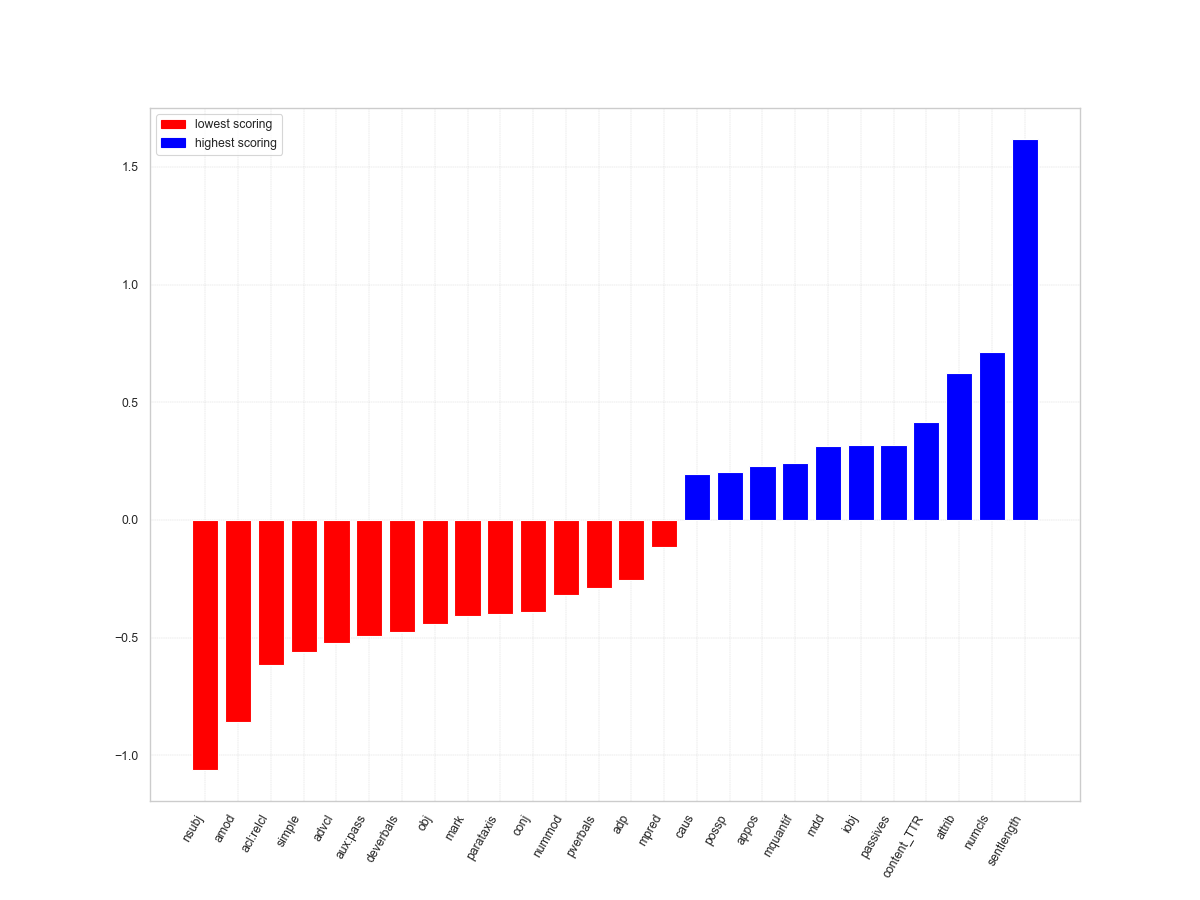
\includegraphics[width=.85\linewidth]{figures/bad-good-bars-ud26}
	\caption{\label{fig:qua-weights}Weights loading the decision towards each category for 26 RFECV-selected items}	
\end{figure}
Figure~\ref{fig:qua-weights} visualises the contribution of each feature to the improved classifier. 

We omitted the analysis of QuEst++ features on this dataset due to its poor performance, which was even lower than the random baseline.

Concluding the observations from the experiments on document labels, let us see whether there were commonalities between the outcomes of professionalism and quality classifications. Despite the classification results on UD features were higher in professional variety classification than in translation quality classification (79.39\% vs 68.9\% on the best-performing subsets of features), we would argue that translationese is more related to quality than to professionalism. Analysis in Sections~\ref{ssec:var} (page~\pageref{pg:more_professional_more_translated}) demonstrated that some translationese features were actually more typical to professional translations than to student translations. This finding was against our expectations, but helped the classifier. 
However, quite in line with the expected, the properties of \textit{bad} translations on most translationese features indicated that these translations had major deviations from the expected TL norm. %, mostly because they carried over ST features. 
%There were only two strong translationese predictors that worked for predicting both varieties and quality: (\hyperlink{acl:relcl}{relative clauses}, \hyperlink{mark}{subordinate clause introducers}).
%Interestingly, there were two features that were useless for any translationese classification among the other six features shared by professionalism and quality classifiers (\hyperlink{appos}{paranthetical modifiers of nouns}, \hyperlink{conj}{syntactic conjuncts}).  % we are talking here about the intersection of \hyperlink{wd:15best-var}{15} and 26 features.
\label{pg:bad_tendencies}
It means that distinctions between professional varieties and quality categories run along different directions. \textbf{Professional translations do not necessarily exhibit less translationese than student translations, while lower-ranking translations do demonstrate stronger translationese tendencies.} In particular, \textit{bad} translations feature longer sentences, more complex sentence structure (more clauses, especially relative clauses), lower TTR, more analytical passives and fewer passive constructions, more nouns functioning as subjects, more modal predicates, more verbal forms, including overuse of copula verbs, de-verbal nouns and participles. 

% Following the suggestion by~\ref{Aharoni2015} who relied on boolean vectors reflecting usage of PoS, listed function words and context free grammar rules to predict MT quality, we implemented an additional SVM quality classifier using probabilities for translated class from student translationese classification on best-performing features as a single input. This classifier achieved F1-score of ???? for `bad' vs `good' experiment.

%Inspired by \cite{Aharoni2014} results for French-English MT, showing that the higher the translationese classification accuracy, the lower the expected translation quality, this research applies a similar approach in the domain of human English-to-Russian translation.

\section{\label{sec:_scores}Regression Tasks}
The purpose of this section is to compare the performance of SVM on document-level datasets with two types of quality scores: a score derived from error annotation and a score obtained through direct assessment.

We want to find out which approach to benchmarking quality by human judges is better aligned with the objective properties of translations as captured by our representations, with a focus on the established translationese indicators.

\subsection{\label{ssec:my_doc_regressors}Experimental Setup}

\paragraph{Datasets} 
The input for the quality prediction tasks, formulated as regression problems, was stored in a separate table of the structure similar to the dataset with document-level labels. It included instances in rows and features in columns. All tested scores, sentence-aligned documents and their lemmatised versions were added as columns as well. 
%It included the total of 1106 instances (rows). 
The intersection between quality-labelled and quality-scored student translations included about 17\% of the total number of unique student translations used in this thesis (206 of 1222 documents). 
Therefore, the datasets were kept separate.

In brief, the error-annotated subcorpus consists of 553 parallel documents, 140 of which are also annotated with DA scores. Both collections include multiple translations for 46 and 30 STs, respectively.
The quality scores were generated as described on page~\pageref{pg:tq} in Section~\ref{ssec:err} for error-based scores and on page~\pageref{pg:final_da} in Section~\ref{ssec:da} for scores from direct assessment. 
In particular, the quality scores included:
\begin{description}\compresslist{}
	\item[accuracy:] frequency of content errors weighted for error categories and normalised to the ST word count;
	\item[fluency:] frequency of language errors weighted for error categories and normalised to the ST word count;
	\item[tq:] overall quality score and its variant (\textbf{scaled\_tq}) transformed into the 0-100 range;
	% as follows scaled_score = (((100 - 0) * (score_current - minscore)) / (maxscore - minscore)) + 0
	\item[da\_mean:] document-level scores from DA averaged from sentence-level and their z-transformed variant (\textbf{da\_zmean})
\end{description}

\paragraph{Representations}

We used the same representations as for the labelled datasets. 
Given the poor performance on \textit{collgram}- and \textit{ngram}-based features and on \textit{stsb-xlm-r-m} vectors in the classification tasks, we omit them from the results in regression experiments reported in this section. 
% this is a bad decision if we contend that error-based scores have a different perspective on quality.

\paragraph{Learning algorithm and evaluation setup}
% regressor = SVR(kernel='rbf', degree=3, gamma='scale', coef0=0.0, tol=0.001, C=1.0, epsilon=0.1, max_iter=-1, shrinking=True)
For translated documents with quality scores, the ML task is formulated as a regression problem. We learn the target scores using \gls{SVR} as implemented in \textit{scikit-learn}, with the library default settings. In particular, the algorithm uses \textit{radial basis function (rbf)} kernel, with \textit{gamma} parameter set to `scale', \textit{C} to 1.0 and \textit{epsilon} to 0.1.
We omit the results for the neural regressor, because they are not different from SVR performance in a principled way as was the case in Sections~\ref{sec:detect}, \ref{ssec:var} and~\ref{ssec:bin}.

The performance of \gls{SVR} is reported in terms of Spearman's rank correlation coefficient (r) and \gls{RMSE}. The former is selected because the quality scores are not normally distributed especially at sentence level (see Figures~\ref{fig:sents_weighed_aspects} and~\ref{fig:sents_tq} at page~\pageref{pg:skews} in Chapter~\ref{cha:quest}). \gls{RMSE} helps to keep track of the magnitude of errors in predicted scores. This metric is typically used in the quality estimation shared tasks by \gls{WMT}.

\paragraph{Feature analysis methods}
The strength of the relationship between each variable (feature) and target labels was measured using 5-fold cross-validated \textit{linear regression} which returned Spearman's correlation coefficient for continuous response variable (scores) in a regression task. 

% MAE measures the average magnitude of the errors in a set of predictions, without considering their direction. It’s the average over the test sample of the absolute differences between prediction and actual observation where all individual differences have equal weight.

%RMSE is a quadratic scoring rule that also measures the average magnitude of the error. It’s the square root of the average of squared differences between prediction and actual observation.

% Since the errors are squared before they are averaged, the RMSE gives a relatively high weight to large errors. This means the RMSE should be more useful when large errors are particularly undesirable. 

% Both MAE and RMSE express average model prediction error in units of the (dependent) variable of interest. Both metrics can range from 0 to ∞ and are indifferent to the direction of errors. 

% They are negatively-oriented scores, which means lower values are better.

% RMSE has a tendency to be increasingly larger than MAE as the test sample size increases
% This can problematic when comparing RMSE results calculated on different sized test samples, which is frequently the case in real world modeling.

% RMSE increases as the variance associated with the frequency distribution of error magnitudes also increases. RMSE does not necessarily increase with the variance of the errors. RMSE increases with the variance of the frequency distribution of error magnitudes.
\subsection{\label{ssec:doc_err_res}Document Level: Error-based Scores}
Based on the existing error annotation, we generated three quality scores. Accuracy and fluency score were calculated from content and language error frequencies, respectively. Overall translation score (tq) was obtained using raw overall error statistics. All scores were normalised to the ST word count.
In an attempt to generate more theoretically justified scores, we also produced a weighted version of these scores using an elaborate weighting scheme. \textit{Weighted} accuracy and fluency scores in Table~\ref{tab:docs_err_par} take into account severities of errors (e.g. a critical error weights more than a minor error). Additionally, these scores are weighted by individual categories of content and language errors as recommended by \textit{TAUS}. For example, an error in collocation has a greater weight than a spelling error. 
The overall quality score uses the severities and annotated positive assessment (kudos) in its weighted variant. This explains why tq score can go over the maximum bound of the absolute scale (100). Scaled tq score is tq score re-calculated for a 0-100 scale, using Formula~\ref{eq:squeezeit}:
\begin{equation}\label{eq:squeezeit}
\begin{split}
scaled score = \frac{100\times (score - min)}{max - min} \\
\end{split}
\end{equation}
where \textit{score} is normalised error frequency, \textit{min} and \textit{max} are respective values of the unscaled score range.

The scaling was done to put the scores from error annotation on the same measuring scale as DA scores. Detailed account of converting error statistics to scores is given in Section~\ref{ssec:err} (see page~\pageref{pg:err-score-generation}). 

Table~\ref{tab:docs_err_par} has the parameters of each quality score distribution (across 553 translations). Note that weighted scores are better distributed across the 0-100 scale, while unweighted scores are hurdled around the maximum value.
\begin{table}[H]
	\centering
	\begin{tabular}{l|ccc}
		\toprule
		& Min   & Max    & Mean (+/-STD)  \\
		\midrule
		\multicolumn{4}{c}{Unweighted scores} \\
		\midrule
		accuracy   & 93.55 & 100    & 98.12 (+/-1.04)  \\
		fluency    & 90.88 & 99.8   & 97.36 (+/-1.32)  \\
		tq         & 87.62 & 99.56  & 95.49 (+/-1.92)  \\
		scaled\_tq & 0     & 100    & 65.86 (+/-16.04) \\
		\midrule
		\multicolumn{4}{c}{Weighted scores} \\
		\midrule
		accuracy   & 61.28 & 98.9   & 86.03 (+/-6.69)  \\
		fluency    & 59.21 & 98.46  & 86.52 (+/-6.11)  \\
		tq         & 72.67 & 100.36 & 92.69 (+/-4.35)  \\
		scaled\_tq & 0     & 100    & 72.3  (+/-15.72) \\
		\bottomrule
	\end{tabular}
	\caption{\label{tab:docs_err_par}Quantitative parameters of error-based scores across 553 documents}
\end{table}

Table~\ref{tab:doc_err_double} has the results of the document-level regression tasks for the error-based scores across seven representation.
\paragraph{\label{pg:doc_err_ud_vs_all}Performance of UD against other representation}
Similar to classification experiments on quality labels, morphosyntactic features, proposed in this thesis, were significantly outperformed only by \textit{mdeberta3} on unweighted accuracy and tq scores, and by \textit{mdeberta3} and \textit{ruRoberta} on fluency.
The highest result of $r=0.67$ was seen on \textit{mdeberta3} representations for weighted overall quality (cf. $r=0.45$ for UD features). % not significantly outperformed in any other setting
As expected, \textit{collgram} and \textit{ngram} features implicitly present in \textit{all} were not helpful and introduced noise, showing slightly lower performance than UD feature set across all scores. 
Interestingly, a custom \textit{tf-idf} representation\wlvfootnote{produced on lemmatised corpus with proper names and numbers substituted with respective placeholders, see page~\pageref{pg:tfidf_meth}} consistently performed better than both morphosyntactic features and TQ-estimation-dedicated cross-lingual sentence embedding model from \textit{TransQuest} in absolute terms, but we do not have enough data to see statistically significant results on these comparisons.

\begin{table}[H]
	\centering
	\begin{tabular}{l|cl|cl|cl|cl}
		\toprule
		& \multicolumn{2}{c|}{accuracy} & \multicolumn{2}{c|}{fluency}  & \multicolumn{2}{c|}{tq} & \multicolumn{2}{c|}{scaled\_tq}    \\
		\midrule
		\multicolumn{9}{c}{Unweighted scores} \\
		\midrule
		       & \textit{r}  & RMSE & \textit{r}  & RMSE & \textit{r}  & RMSE & \textit{r} & RMSE  \\
		\midrule
			UD     & \textbf{0.43} & 0.95 & \textbf{0.43} & 1.18 & \textbf{0.45} & 1.72 & 0.32 & 15.5  \\
			all             & 0.41 & 0.96 & 0.43 & 1.19 & 0.43 & 1.74 & 0.32 & 15.56 \\
			quest61         & 0.37 & 0.98 & 0.42 & 1.16 & 0.36 & 1.73 & 0.31 & 15.22 \\
			\midrule
			tfidf           & 0.48 & 0.92 & 0.49 & 1.14 & 0.47 & 1.69 & 0.39 & 15.59 \\
%			\midrule
			TQmono-m        & 0.46 & 0.94 & 0.47 & 1.15 & 0.45 & 1.68 & 0.35 & 15.3  \\
			ruRoberta & 0.51 & 0.91 & 0.53 & 1.08 & 0.54 & 1.57 & 0.44 & 14.84 \\
			mdeberta3  & 0.58 & 0.87 & 0.58 & 1.05 & 0.62 & 1.5  & 0.56 & 14.62 \\
		\midrule
		\midrule
		\multicolumn{9}{c}{Weighted scores} \\
		\midrule
		UD              & 0.38 & 6.31 & 0.37 & 5.72 & 0.44 & 4.02 & \textbf{0.38} & 15.13 \\
		all             & 0.38 & 6.34 & 0.35 & 5.77 & 0.43 & 4.06 & 0.36 & 15.18 \\
		quest61         & 0.32 & 6.34 & 0.33 & 5.68 & 0.37 & 4.1  & 0.33 & 15.13 \\
		\midrule
		tfidf           & 0.4  & 6.36 & 0.39 & 5.78 & 0.48 & 4.04 & 0.45 & 15.23 \\
%		\midrule
		TQmono-m        & 0.4  & 6.13 & 0.37 & 5.64 & 0.47 & 3.92 & 0.38 & 14.85 \\
		ruRoberta & 0.48 & 5.98 & 0.45 & 5.47 & 0.57 & 3.74 & 0.5  & 14.53 \\
		mdeberta3  & \boxit{0.3in}0.62 & 5.76 & \boxit{0.3in}0.59 & 5.21 & \boxit{0.3in}0.67 & 3.54 & \boxit{0.3in}0.63 & 14.19 \\
		\bottomrule
	\end{tabular}
\caption{\label{tab:doc_err_double}Regression results for error-based quality scores (553 documents). For each quality score, the boldface type is used to denote the highest $r$ for manual features; the highest $r$ for content-dependent representations is boxed}
\end{table}

Table~\ref{tab:doc_err_double} omits STD values for brevity. These values for $r$ vary in the following ranges across representations: accuracy (0.07--0.10), fluency (0.09--0.12), tq (0.08--0.13), scaled\_tq (0.06--0.12).

\paragraph{Comparison of regressors across types of scores}
From Table~\ref{tab:doc_err_double}, Spearman's \textit{r} was higher for overall quality score (tq) than for accuracy, fluency or scaled\_tq for both weighted and unweighted versions. However, most differences between the results on accuracy, fluency or tq were not statistically significant. Whenever there was a significant difference (mostly between weighted fluency and tq), the results were always better for tq.

Significant differences between weighted and unweighted versions were seen only for fluency on \textit{ruRoberta} and for scaled\_tq on \textit{mdeberta3}. However, it is impossible to say which version of scores was more learnable because the unweighted score returned higher results in the former setting and the weighted score was superior in the latter. 
It is noteworthy that weighted scores returned much larger error between the gold scores and predictions as measured by \gls*{RMSE}. 
Based on these observations, {unweighted scores are preferable to weighted scores}.

\textbf{Scaled version of the overall quality scores was inferior to unscaled version} on almost all representations. % for all representations except \textit{mdeberta3} on unweighted scores. 
Scaling the quality score tripled the average prediction error, too.
In the subsequent experiments reported in this chapter, weighted scores and scaled version of overall quality (scaled\_tq) are excluded from the analysis.

These results draw attention to a curious finding. Contrary to the expectations, we did not see statistically significant differences between accuracy and fluency in terms of performance on any representations, including translationese features. If these scores captured independent aspects of quality, we would expect higher results for fluency on our TL-centred representations. We can cautiously suggest that \textbf{our data did not contain translations that were very inaccurate but fluent, and vice versa}. The two aspects of quality seem to be correlated. Indeed, on weighted scores, Spearman's correlation coefficient between them was 0.897\wlvfootnote{Intuitively, the weighted scores, which take into account the type of errors and their severities, reflect the actual opinion of assessors' on quality}. % $r=0.309$ on unweighted scores based on simple normalised frequency of content and language errors disregarding severities or subtypes of these major categories
This might mean that \textbf{an \gls*{HTQE} approach aimed at fluency can be a useful proxy for overall document-level quality from error annotation}.
Another explanation is lack of training data. Our experiments were run on 553 annotated translations and did not reveal the differences between the two aspects of quality. If more data is needed to reveal these differences, then the differences must be really small. 
%A more plausible explanation is that \textbf{scores from error annotation do not reflect translationese properties of translations, at least when they are generated for entire documents}. %; language errors are focused on other imperfections of student translations. 

\paragraph{Feature analysis} 
Feature selection for UD set did not yield any sizeable improvements in performance on either weighted or unweighted scores. 
On weighted scores, the maximum gain was for accuracy, where the value for correlation coefficient went up from 0.38 to 0.42 on a selection of 29 features. On unweighted scores, a selection of 44 UD features increased the regression result on accuracy only by 0.01 (from 0.43 to 0.44). 

Limiting QuEst++ feature set to the best-performing 21 features resulted in a very modest gain of 0.03 on accuracy. % on random 140 docs 9 QuEst++ achieve the same result: ['bqe_1009', 'qe_1026', 'qe_1032', 'bqe_1053', 'bqe_1054', 'bqe_1074', 'qe_9994', 'qe_9995', 'qe_9996']
No selection of features was able to improve the performance on fluency and tq scores for either UD or QuEst++. 

To reveal the features that were better correlated with various quality scores, we used each of them as a single input to a \textit{linear regression} algorithm as implemented in \textit{scikit-learn}, with the library default parameters.  % Logistic regression is switched to linear regression because we use continuous instead of categorical quality estimate

Univariate correlation analysis did not reveal any features from UD, collgram, ngram or QuEst++ feature sets that were associated with any quality score for more than Spearman's $r=0.274$. % Interestingly, the values of $r$ between any single feature and (best-performing) fluency scores were more than 1.5 times lower than for accuracy or tq. % I am not sure how to explain this.
% the highest r (positive or negative seen for collgram, ngram was on unweighted tq: bigram-tscore_std   0.189) 
\label{pg:scores_not_translationese}
Despite the correlation between the proposed quality indicators and various quality scores was small, we noticed that some important quality predictors from UD features (from the top 10 better-correlated features) contributed to all scores while others remain specific to accuracy or fluency. The intersection of top 10 features by correlation with unweighted accuracy, fluency and tq included \textit{nsubj, acl:relcl, obj}. These relatively strong predictors shared by all error-annotated scores capture syntactic complexity of sentences in translations: number of explicit syntactic subject and object dependencies across all clauses (\textit{nsubj}, \textit{obj} and number of relative clauses (\textit{acl:relcl})). All of them were weakly but positively correlated with the scores. This brings us to a counter-intuitive conclusion that the more well-developed finite clauses there were in the sentence, the higher was the quality score. This also contradicts the results on binary labels (see page~\ref{pg:bad_tendencies}).

One way to interpret this contradiction is to suggest that holistic document-level perception of quality incorporated translationese-related properties of translations, while error-based quality scores, even from fluency errors, did not reflect translation solutions that can be explained by translationese. 
The fact that prominent quality predictors were equally associated with accuracy, fluency and tq, together with the observation that this association was weak ($r<0.243$), confirms that even if accuracy and fluency reflected different aspects of translation quality, these aspects were not related to translationese.

\label{pg:errors_some_coherence_with_translationese_theory_of_quality}
A look at other translationese features that were found among the top 10 by correlation with either accuracy or fluency suggests an interpretation coherent with the translationese hypothesis of quality for some of them. 
For example, accuracy scores returned $r=0.226$ for Spearman's correlation with the frequency of negative particles. This aligns well with the translationese explanation: the more negative particles, the higher the translation quality. Less fluent translations tend to underuse negative constructions and follow the English affirmative way of expression. Accuracy scores also had $r=-0.1$ correlation with epistemic markers. The overuse of literal translations for the phrases like \textit{certainly, as far as we know, of course, no doubt, it appears that}, which are more common in English, seemed to predict lower-ranking translations. The most prominent indicator of fluency was the frequency of modal predicates ($r=-0.106$). From translationese theory perspective, the overuse of modal predicates in English-to-Russian translation signals lower quality.
Even if these observations are acceptable, they do not explain either error-based scores or the difference between them convincingly due to their low potency.   

\label{pg:quest_feats4err}
The comparable \textbf{performance of QuEst++ for all error-based scores was based on ST complexity features}.
For the QuEst++ feature set, the intersection between best-performing features on accuracy and fluency included six out of 10 top features. Five of them were complexity (ST-based) features that \textit{measured average number of translations per source word} counted with various Giza probability thresholds (including \#1016, \#1018, \#1020, \#1022, \#1024, e.g. document-level QuEst++ feature \#1024: ``average number of translations per source word in the sentence (threshold in giza1: prob > 0.05)''). Apart from that, number of sentences in the target document (\#9801) was relatively well correlated with all scores. It indicated that the more sentences there were in a translation, the higher was the quality score.
The error-annotated dataset included multiple translations for 47 English sources. Apparently, the differences between them were most contributive to the QuEst++ regressor performance. We looked through the extended lists of top 15 most-associated features for accuracy and fluency, and found that they represented the properties of ST (with the exception of two adequacy features). Over-reliance of this classifier on the ST side fits well with no distinction between accuracy and fluency. Indeed, a more demanding ST can trigger both content and language errors, as we demonstrated in~\cite{Kunilovskaya2022err}.
However, it also shows that QuEst++ feature set did not pick up any relevant distinctions between translations per se. 
%Analysis of intersections in \textit{tf-idf} top features did not reveal any patterns and was not enlightening. 

%fluency	
%qe_1024	average number of translations per source word in the document (threshold in giza1: prob > 0.5)
%qe_9801	Number of sentences in the source document
%qe_1016	average number of translations per source word in the sentence (threshold in giza1: prob > 0.01)
%bqe_1001	number of tokens in the source document
%qe_1018	average number of translations per source word in the sentence (threshold in giza1: prob > 0.05)
%qe_1020	average number of translations per source word in the sentence (threshold in giza1: prob > 0.10)
%bqe_1022	average number of translations per source word in the sentence (as given by IBM 1 table thresholded so that prob(t|s) > 0.2)
%bqe_1046	average unigram frequency in quartile_1 of frequency (lower frequency words) in the corpus of the source document
%qe_1059	percentage of distinct bigrams seen in the source corpus (in all quartiles) - document-level
%qe_1004	no tokens in the target / no tokens in the source
%qe_1026	average number of translations per source word in the document (threshold in giza1: prob > 0.01) weighted by the frequency of each word in the source corpus")
%qe_1032	average number of translations per source word in the document (threshold in giza1: prob > 0.2) weighted by the frequency of each word in the source corpus")
%qe_1093	ratio of percentage of verbs in the source and target documents
%
%accuracy	very 
%qe_1056	average trigram frequency in quartile 3 of frequency (lower frequency words) in the corpus of the source document
%qe_1085	ratio of percentage of content words in the source and target documents
%qe_1089	percentage of verbs in the source document
%qe_1052	average bigram frequency in quartile 3 of frequency (lower frequency words) in the corpus of the source document
%bqe_1050	average bigram frequency in quartile 1 of frequency (lower frequency words) in the corpus of the source document
%qe_1093	ratio of percentage of verbs in the source and target documents
%qe_1024	average number of translations per source word in the document (threshold in giza1: prob > 0.5)
%qe_9801	Number of sentences in the source document
%qe_1016	average number of translations per source word in the sentence (threshold in giza1: prob > 0.01)
%qe_1018	average number of translations per source word in the sentence (threshold in giza1: prob > 0.05)
%qe_1020	average number of translations per source word in the sentence (threshold in giza1: prob > 0.10)
%bqe_1022	average number of translations per source word in the sentence (as given by IBM 1 table thresholded so that prob(t|s) > 0.2)

% for weighted scores
% Selected accuracy features 29: ['addit', 'anysome', 'content_dens', 'deverbals', 'finites', 'infs', 'interrog', 'mhd', 'mpred', 'nn', 'nnargs', 'numcls', 'passives', 'ppron', 'pverbals', 'sconj', 'simple', 'wdlength', 'advcl', 'amod', 'aux:pass', 'case', 'fixed', 'flat', 'nmod', 'nsubj', 'nummod', 'obj', 'obl']

% Selected fluency features 12: ['anysome', 'deverbals', 'finites', 'neg', 'nn', 'passives', 'simple', 'advcl', 'appos', 'case', 'fixed', 'obj']
% Selected tq features 21: ['anysome', 'deverbals', 'finites', 'interrog', 'neg', 'nn', 'nnargs', 'passives', 'ppron', 'sentlength', 'simple', 'wdlength', 'advcl', 'amod', 'aux:pass', 'case', 'conj', 'fixed', 'nmod', 'nsubj', 'obl']

\subsection{\label{ssec:doc_da_res}Document Level: Direct Assessment}
Our annotation setup for perceived quality was sentence-level, and document-level scores were obtained by averaging sentence scores. Recall that the annotation setup did not present sentences in isolation. Instead, the raters could see the entire parallel document. They were asked to read the ST before annotation. 

In the description below, \textit{da\_mean} stands for the mean raw score between the raters. 
Following the practice adopted in \gls{WMT} quality estimation shared tasks, raw scores were standardised by rater using z-transformation and then averaged to obtain \textit{da\_zmean} scores. % NB! from WMT 2021: DA scores are standardised using the z-score by rater. Participating systems are required to score sentences according to z-standardised DA scores.

Also, as explained in Section~\ref{ssec:da}, there were only two admissible ratings from six sentence-wise cross-annotations of 140 documents due to strict thresholds for internal rater reliability. 
%Ten documents were discarded because their annotations were incomplete or there were other technical problems preventing the recovery of trustworthy results. 
The level of agreement between the two selected ratings in terms of Spearman's rank correlation co-efficient for document-level scores was 0.503 (p < 0.05). % z-transform does not play a role in calculating this correlation

% this is double-checked with the output of python3 get_input_tables/1_scores_doc_concatenator.py --err_type unweighted --da_type 2raters
\begin{table}[H]
	\centering
	\begin{tabular}{l|ccc|ccc}
		\toprule
				& \multicolumn{3}{c|}{unweighted} & \multicolumn{3}{c}{weighted} \\
		\midrule
		& accuracy   & fluency & tq    & accuracy & fluency & tq    \\
		\midrule
		da\_mean & 0.509      & 0.169   & 0.391 & 0.514    & 0.408   & 0.559 \\
		\bottomrule
	\end{tabular}
\caption{\label{tab:doc_err-da_corr}Spearman's $r$ between DA scores and quality scores from error annotation}
\end{table}

Table~\ref{tab:doc_err-da_corr} has the Spearman's correlation of averaged DA score (da\_mean) and the three major scores from error annotation. All results are significant at the confidence level of 5\%.

It can be seen from Table~\ref{tab:doc_err-da_corr} that weighted error-based scores were better aligned with perceived quality. To an extent, it justifies the error weighting scheme based on error categories and severities. Perceived quality (DA scores) were more correlated with accuracy and overall scores than with fluency. It means that the \textbf{raters penalised content errors more than language errors}. 

\begin{table}[H]
	\centering
	\begin{tabular}{l|ccc}
		\toprule
		& Min   & Max    & Mean (+/-STD)          \\
		\midrule
		da\_mean  & 56.36 & 95.57 & 83.65 (+/-7.99) \\
		da\_zmean & -3.10 & 1.34  & 0.00 (+/-0.88) \\
		\bottomrule
	\end{tabular}
	\caption{\label{tab:doc_da_dist}Document-level: Parameters of DA scores distribution}
\end{table}
% unique values 140

The resulting distribution of scores from DA annotation for 140 documents (averaged from sentence scores) has the parameters reflected in Table~\ref{tab:doc_da_dist}. They are also visualised in Figure~\ref{fig:da_scores} on page~\pageref{pg:da_score_hists}. The distribution of DA scores is skewed to the right. 

According to the results, presented in Table~\ref{tab:da_doc_res}, there was no consistent differences between the performance of the regressors on raw mean DA scores and on mean z-transformed scores. In fact, none of the differences between the two \textit{r} columns in Table~\ref{tab:da_doc_res} were statistically significant.
%In our setting, it indicates that the raters did not differ much in how they used the assessment scale. Their judgments were well-calibrated. % Actually the RMSE for the scores returned by the two raters was 

\begin{table}[H]
	\centering
	\begin{tabular}{l|cl|cl}
		\toprule
		& \multicolumn{2}{c|}{da\_mean} & \multicolumn{2}{c}{da\_zmean} \\
		\midrule
		rep             & \textit{r}         & RMSE & \textit{r}          & RMSE \\
		\midrule
%		\multicolumn{5}{c}{harmonised 2 raters}     \\tab:doc_err-da_corr
%		\midrule
%			ud              & 0.21 & 7.68 & 0.13 & 0.54 \\
%			all             & 0.2  & 7.69 & 0.23 & 0.52 \\
%			quest61         & 0.18 & 7.84 & 0.09 & 0.58 \\
%			tfidf           & 0.17 & 7.93 & 0.18 & 0.52 \\
%			TQmono-m        & 0.21 & 7.7  & 0.27 & 0.51 \\
%			ruRoberta & 0.18 & 7.76 & 0.22 & 0.52 \\
%			mdeberta3  & 0.35 & 7.62 & 0.29 & 0.5   \\
%		\midrule
%		\multicolumn{5}{c}{2raters}     \\ 
%		\midrule
            UD        & \textbf{0.23} (+/-0.25) & 7.27 (+/-1.92) & 0.16 (+/-0.23) & 0.81 (+/-0.19) \\
			all       & 0.21 (+/-0.21) & 7.29 (+/-1.93) & \textbf{0.23} (+/-0.26) & 0.79 (+/-0.20) \\
			quest61   & 0.18 (+/-0.22) & 7.44 (+/-1.90) & 0.11 (+/-0.27) & 0.88 (+/-0.17) \\
			\midrule
			tfidf     & 0.19 (+/-0.26) & 7.56 (+/-1.93) & 0.20 (+/-0.23) & 0.79 (+/-0.17) \\
			TQmono-m  & 0.23 (+/-0.20) & 7.31 (+/-1.74) & 0.22 (+/-0.20) & 0.78 (+/-0.16) \\
			ruRoberta & 0.22 (+/-0.27) & 7.35 (+/-1.91) & 0.23 (+/-0.22) & 0.78 (+/-0.18) \\
			mdeberta3 & \boxit{0.3in}0.37 (+/-0.20) & 7.22 (+/-1.89) & \boxit{0.3in}0.32 (+/-0.22) & 0.75 (+/-0.18) \\
%		\midrule
%		\multicolumn{5}{c}{3raters}   \\
%		\midrule
%			ud              & 0.2  & 6.22 & 0.23 & 0.55 \\
%			all             & 0.25 & 6.19 & 0.29 & 0.52 \\
%			quest61         & 0.19 & 6.35 & 0.05 & 0.61 \\
%			tfidf           & 0.14 & 6.47 & 0.13 & 0.55 \\
%			TQmono-m        & 0.17 & 6.3  & 0.21 & 0.55 \\
%			ruRoberta & 0.1  & 6.36 & 0.22 & 0.54 \\
%			mdeberta3  & 0.26 & 6.26 & 0.21 & 0.53 \\
%		\midrule
%		\multicolumn{5}{c}{6raters}  \\
%		\midruler
%			ud              & 0.09 & 4.89 & 0.13 & 0.52 \\
%			all             & 0.2  & 4.88 & 0.25 & 0.5  \\
%			quest61         & 0.13 & 4.92 & 0.19 & 0.53 \\
%			tfidf           & 0.22 & 4.88 & 0.23 & 0.49 \\
%			TQmono-m        & 0.33 & 4.79 & 0.3  & 0.5  \\
%			ruRoberta & 0.22 & 4.84 & 0.26 & 0.51 \\
%			mdeberta3  & 0.3  & 4.74 & 0.33 & 0.47 \\
		\bottomrule
	\end{tabular}
\caption{\label{tab:da_doc_res}Document-level: Regression results with STD for DA scores (140 documents). The highest $r$ for each score by manual features and content-dependent regressors are highlighted}
\end{table}

Further on, there were no statistically significant differences between the representations shown in rows, either. Although we can observe that the value for Spearman's $r$, averaged across 10 folds of the experiment, was higher for \textit{mdeberta3}, the performance of the regressor was very volatile from fold to fold, ranging from $r=0.068$ to $r=0.758$. In particular, Spearman's $r$ values across 10 runs of the \textit{mdeberta3} regressor on \textit{da\_mean} scores were: [0.179, 0.385, 0.464, 0.389, 0.666, 0.244, 0.759, 0.301, 0.275, 0.068].
%\todo[inline]{An suggests reporting res for folds} 

We have to conclude that none of the representations was more successful than the other in learning DA scores. Clearly, this is the effect of small training data (140 documents) in conjunction with no strong signal coming from any attempted representations. 

\begin{table}[H]
	\centering
	\begin{tabular}{l|cl|cl|cl|cl}
		\toprule
		& \multicolumn{2}{c|}{accuracy} & \multicolumn{2}{c|}{\textbf{fluency}}  & \multicolumn{2}{c|}{tq} & \multicolumn{2}{c}{scaled\_tq}    \\
		\midrule
		\multicolumn{9}{c}{Unweighted scores} \\
		\midrule
		& \textit{r}        & RMSE & \textit{r}       & RMSE & \textit{r}    & RMSE & \textit{r}    & RMSE  \\
		\midrule
		UD                & 0.13  & 1.32 & \textbf{0.4}     & 1.48 & 0.24  & 2.48 & 0.21       & 20.62 \\
		all               & 0.02  & 1.34 & 0.33    & 1.51 & 0.14  & 2.5  & 0.13       & 20.66 \\
		quest61           & -0.07 & 1.46 & 0.39    & 1.47 & 0.15  & 2.47 & 0.1        & 20.59 \\
		\midrule
		tfidf             & 0.07  & 1.3  & 0.45    & 1.48 & 0.22  & 2.42 & 0.21       & 20.59 \\
%		\midrule
		TQmono-m          & 0.01  & 1.38 & 0.42    & 1.46 & 0.24  & 2.42 & 0.2        & 20.54 \\
		ruRoberta   & 0.04  & 1.38 & 0.45    & 1.41 & 0.25  & 2.37 & 0.29       & 20.31 \\
		mdeberta3    & 0.52  & 1.12 & \boxit{0.3in}0.54    & 1.35 & 0.52  & 2.1  & 0.46       & 19.93 \\
%		\midrule
%		\midrule
%		\multicolumn{9}{c}{Weighted scores} \\
%		\midrule
%		UD                & 0.1   & 9.14 & 0.23    & 7.68 & 0.17  & 5.91 & 0.18       & 21.35 \\
%		all               & 0.03  & 9.15 & 0.16    & 7.73 & 0.13  & 5.94 & 0.14       & 21.47 \\
%		quest61           & -0.17 & 9.37 & 0.15    & 7.72 & -0.02 & 6.11 & 0          & 21.53 \\
%		\midrule
%		tfidf             & 0.07  & 9.13 & 0.23    & 7.72 & 0.18  & 5.93 & 0.17       & 21.46 \\
%		\midrule
%		TQmono-m          & 0.1   & 9.11 & 0.24    & 7.64 & 0.21  & 5.92 & 0.21       & 21.46 \\
%		ruRoberta   & 0.09  & 9.17 & 0.3     & 7.56 & 0.15  & 5.93 & 0.2        & 21.32 \\
%		\textbf{mdeberta3}    & \textbf{0.53}  & 8.48 & \textbf{0.5}     & 7.15 & \boxit{0.4in}\textbf{0.58}  & 5.35 & \textbf{0.55}       & 20.69 \\
		\bottomrule
	\end{tabular}
	\caption{\label{tab:err140_res}Regression results on error-based scores for 140 cross-annotated documents. The highest results across all scores by manual features and content-dependent regressors are highlighted}
\end{table}

The results for document-level experiments on DA scores were twice lower than on error-based scores reported in Section~\ref{ssec:doc_err_res} above. To rule out the impact of data size (553 vs 140 documents for error-based and DA scores, respectively), we obtained the error-based results on 140 documents cross-annotated for errors and DA (see Table~\ref{tab:err140_res}).

\textit{Unweighted fluency} was the only error-based score that remained robust on a four times smaller dataset (553 documents vs. 140 documents cross-annotated for errors and DA). The regression results for unweighted fluency were almost twice higher than for mean DA scores on the same dataset, and the differences were statistically significant, unlike the differences between \textit{da\_mean} and accuracy, tq and scaled\_tg in Tables~\ref{tab:da_doc_res} and~\ref{tab:err140_res}.
%\todo[inline]{An suggests unpacking "all other differences"}

It seems that this setup returned the expected higher learnability of fluency, as opposed to accuracy, on the representations limited to the TL-side of the parallel corpora. Besides, it showed that error-based scores seemed to be more consistent and reliable than DA scores. % how do I explain similar performance on accuracy and fluency in a larger dataset? Does it depend on the distribution of scores in the dataset?
 
However, the distributions of accuracy scores in the error-annotated and cross-annotated datasets (see Figure~\ref{fig:acc140binomial} were quite different. In the full dataset, it is close to normal, while in the cross-annotated it is almost binomial. The fluency and tq scores were not as affected by the selection of 140 documents. Recall from Section~\ref{ssec:da} (page~\pageref{pg:intersection140}) that the documents for DA annotation were specifically selected to be in the intersection of error-annotated data and binary quality data. We also aimed to include approximately the same number of \textit{good} and \textit{bad} translations. The observed change in distribution of accuracy scores provides a further confirmation that human judges paid more attention to the accuracy of meaning transfer than to disfluencies in translations. 

\begin{figure}
	\begin{minipage}[c]{0.45\linewidth}
		\centering
		Unweighted accuracy (553 docs)
		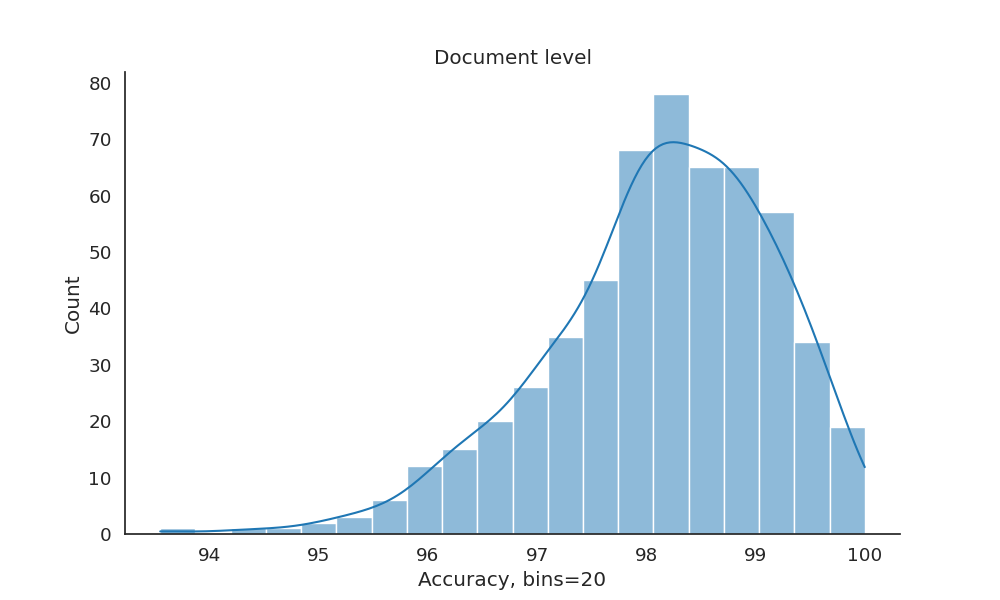
\includegraphics[width=\linewidth]{figures/err/accuracy-distibution-noweights.png}
	\end{minipage}
	\begin{minipage}[c]{0.45\linewidth}
		\centering
		Unweighted accuracy (140 docs)
		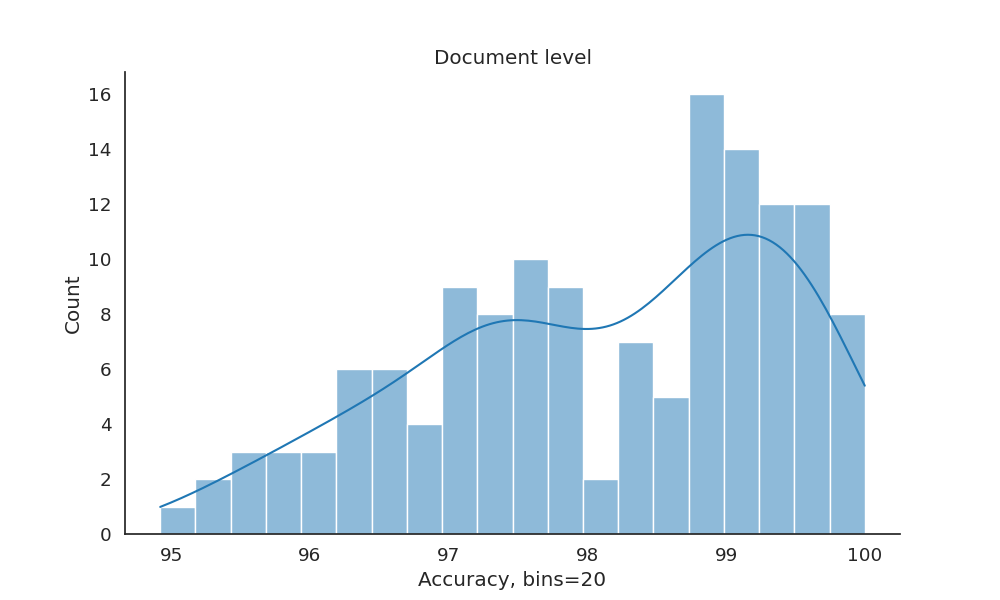
\includegraphics[width=\linewidth]{figures/err/accuracy-distibution-140.png}
	\end{minipage}	
	\caption{\label{fig:acc140binomial}Distributions of accuracy scores for error-annotated and cross-annotated datasets}	
\end{figure}

These details on data selection invalidate the differences in performance between accuracy and fluency on the cross-annotated dataset, while the observation about lack of difference between the two aspects from the point of view of all attempted representations stands. 
This conclusion was confirmed by \textbf{lack of statistical difference between accuracy and fluency} for all attempted representations on a random selection of 140 error-annotated documents. 
The results of this experiment are aggregated in Table~\ref{tab:err140rand_res}.

\begin{table}[H]
	\centering
	\begin{tabular}{l|cl|cl|cl|cl}
		\toprule
		& \multicolumn{2}{c|}{accuracy} & \multicolumn{2}{c|}{fluency}  & \multicolumn{2}{c|}{tq} & \multicolumn{2}{c}{scaled\_tq}    \\
		\midrule
		\multicolumn{9}{c}{Unweighted scores} \\
		\midrule
		& \textit{r}        & RMSE & \textit{r}       & RMSE & \textit{r}    & RMSE & \textit{r}    & RMSE  \\
		\midrule
		UD              & 0.2  & 1.11 & \textbf{0.36} & 1.02 & \textbf{0.36} & 1.72 & \textbf{0.34} & 14.8  \\
		all             & 0.28 & 1.08 & 0.25 & 1.04 & 0.3  & 1.74 & 0.27 & 14.9  \\
		quest61         & \textbf{0.29} & 1.09 & 0.29 & 1.03 & 0.28 & 1.77 & 0.26 & 14.94 \\
		\midrule
		tfidf           & 0.38 & 1.06 & 0.33 & 1.03 & 0.33 & 1.74 & 0.3  & 15.04 \\
%		\midrule
		TQmono-m        & 0.32 & 1.05 & 0.31 & 1.04 & 0.34 & 1.7  & 0.23 & 14.8  \\
		ruRoberta-large & 0.38 & 1.06 & 0.34 & 1.01 & 0.38 & 1.69 & 0.39 & 14.74 \\
		mdeberta3-base  & \boxit{0.3in}0.53 & 0.99 &\boxit{0.3in}0.45 & 0.95 & \boxit{0.3in}0.58 & 1.56 & \boxit{0.3in}0.54 & 14.6 \\
		\bottomrule
	\end{tabular}
	\caption{\label{tab:err140rand_res}Regression results for random 140 documents with error-based scores. For each quality score, the boldface type is used to denote the highest $r$ for manual features; the highest $r$ for content-dependent representations is boxed}
\end{table}

With regard to the \textbf{comparison between error-based and DA scores}, we have seen statistically significant results only for \textit{mdeberta3}, which returned higher results for accuracy, tq and scaled\_tq scores than for da\_zmean scores. 
All other comparisons were inconclusive. Interestingly, \textit{mdeberta3} was exceptional among all representations, including other embedding models. It returned stable and relatively high results regardless the type of error-based score, size of the dataset and distribution of scores. 

%UD features were statistically inferior to \textit{mdeberta3} only in the experiments for accuracy scores.

In sum, the experiments on an random selection of error-annotated documents confirmed \textbf{no difference in regression results for accuracy and fluency on any attempted representations} reported in Section~\ref{ssec:doc_err_res} (see Table~\ref{tab:doc_err_double}). 
We also \textbf{failed to obtain convincing proof that either error-based or DA scores were better aligned with the properties of translation} as represented in this work, except for \textit{mdeberta3} vectors that performed better on accuracy, tq and scaled\_tq scores than on da\_zmean scores. 

\paragraph{Feature analysis} 
We continue to trace the correlation of UD and QuEst++ features with the scores using feature selection and univariate tests, and limiting the analysis to the top ten most successful quality predictors according to both or either of these methods.
In this paragraph, we compared the set of features most associated with error-based scores to the set of features most correlated with DA scores. 

% scores: no statistically significant differences between results on full feature set and on selected features
Feature selection improved the results for \textit{da\_mean} on UD from 0.23 to 0.27 by limiting the feature set to just \textit{deverbals, nmod, nsubj}. The results on QuEst++ went up from 0.18 to 0.24 after limiting the feature set to 24 features. However, we forgo their analysis because the differences were not statistically significant.
%QuEST for da\_mean (24 fets r 0.18 -> 0.24) ['qe_1003', 'bqe_1009', 'qe_1011', 'bqe_1012', 'qe_1013', 'bqe_1015', 'qe_1018', 'qe_1024', 'qe_1028', 'qe_1034', 'bqe_1036', 'qe_1038', 'qe_1044', 'qe_1048', 'qe_1052', 'bqe_1054', 'qe_1055', 'bqe_1074', 'qe_1088', 'qe_1090', 'qe_1091', 'qe_1092', 'qe_1093', 'qe_9994']
\label{pg:da_ignores_translationese_feats}
The analysis of individual correlation of feature values and scores revealed \textbf{a noticeably different set of features correlated with DA scores than with error-based scores for UD and QuEst++}. 
In fact, there was only one UD feature that was in top ten by correlation with DA scores and with three error-based scores (\textit{nsubj}), while \textit{mark, neg, advcl} and \textit{sentlength} were shared with only accuracy or fluency, respectively.
None of these quality indicators support the translationese approach to quality, except, maybe, number of negations (\textit{neg}). If anything, these results mean that the longer and more complex the sentence, the higher the quality. In all likelihood, in \textbf{DA assessment setup translationese properties of texts were ignored by the raters}.  

UD features that were correlated with DA scores (but not with error-based scores) included \textit{mdd, aux, tempseq, aux:pass, mark, copula, advers}. They were positively correlated with DA scores. Higher MDD means higher comprehension difficulty, with sentences requiring additional effort for transforming longer linear distances into syntactic trees at understanding time~\cite[p.162]{Jing2015}. MDD values were greater in translations than in non-translated Russian, inviting a counter-intuitive conclusion that higher complexity correlated with higher quality. Increased frequencies of copula and auxiliary verbs, analytical passives are also signs of more noticeable translationese, which seems to be correlated with higher DA quality. The frequency of adversative discourse markers was negatively correlated with DA scores ($r=-0.224$), i.e. the more explicit markers of contrast were used in a translation, the lower was the perceived quality (e.g. \foreignlanguage{russian}{\textit{однако, несмотря на, тем не менее}} [however, despite, nonetheless]).
\textbf{These observations contradict our assumption that higher-quality translations should show less signs of translationese.}
% trade-off relation between the structural complexity in the two dimensions partially proves the dynamic balance of code-switching from the listener’s and speaker’s perspectives. English tends to reduce the structural complexity in the hierarchical dimension (MHD), while Czech prefers to lessen the processing cost in the linear dimension (MDD).

One common quality indicator among 61 QuEst++ features that cut across all types of quality scores (both DA and error-based) was \textit{the ratio of verbs in the source and target (\#1093)}. It was negatively correlated with the quality, i.e. the fewer verbs in the target, the higher the ratio, and the lower the quality. % which is contrary to what I think 
If anything, this observation contradicts the expectations in the context of English-to-Russian translationese tendencies as was the case with other results for translationese-aware features on error-based (see page~\ref{pg:scores_not_translationese}) and DA scores. Other DA predictors useful for accuracy and tq, or fluency were: 
% tq (\#1052, \#1085), fluency (\#1004)
\begin{description}\compresslist{}
	\item[1052] average bigram frequency in quartile 3 of frequency (lower frequency words) in the source corpus,
	\item[1085] ratio of percentage of content words in the source and target,
	\item[1004] number of tokens in the target over number of tokens in the source.
\end{description}
They were positively correlated with the respective quality scores. 

% discussed on page~\pageref{pg:quest_feats4err} 
Most correlative features that were specific for experiments on DA scores are listed below (in the decreasing order based on individual correlation with \textit{da\_mean} score): 
\begin{description}\compresslist{}
	\item[9992] ratio of word repetitions in target and source documents,
	\item[9993] ratio of lemma repetition between target and source documents,
	\item[1003] ratio of number of tokens in source and target,
	\item[1004] number of tokens in the target over number of tokens in the source,
	\item[1052] average bigram frequency in quartile 3 of frequency (lower frequency words) in the source corpus).
\end{description}

Interestingly, this list primarily includes adequacy features. Recall that error-based scores had ST complexity parameters as major quality predictors. 
Lack of intersection between error-based quality predictors and DA quality predictors from two interpretable feature sets make us conclude that these \textbf{types of assessment reflect dissimilar aspects of translation quality} or our feature sets are incomplete. 
Admittedly, this feature analysis has limited reliability, given weak association of any individual features with the DA scores (maximum $r=0.274$ for negative particles from UD feature set) and the general poor performance of any feature set on DA scores. 
However, the interpretation of most correlative features indicates that \textbf{DA method does not reflect translationese properties of document}.

\subsection{\label{ssec:sent_level}Sentence Level: Error-based and DA Scores}
Given that error-based and DA scores originated at sentence level, we extended these experiments to the sentence-level version of the dataset. It included 3,224 sentences from 140 documents with error-based and DA scores. At sentence level, the distribution of scores was not as affected by the selection of a polarised smaller sample and remained heavily right-skewed for all scores as shown in Figure~\ref{fig:sents_tq} (page~\pageref{fig:sents_tq}). Nonetheless, we report results on randomly selected 3,224 sentences. The stack of experiments was run only for unweighted scores. For consistency, we present the results on the full dataset spanning 12,369 sentences, too.

At sentence level, there was enough data to establish that \textbf{translationese-aware features were relatively competitive only for fluency scores}. On the full dataset, they were outperformed for this type of quality only by \textit{ruRoberta} and \textit{mdeberta3}. For accuracy and tq, translationese-aware feature set was inferior to all other representations, including \textit{quest70} ()a dedicated sentence-level QuEst++ feature set), \textit{tf-idf} and \textit{TQmono-m} in addition to \textit{ruRoberta} and \textit{mdeberta3}. This inferiority was lost on 3,224 sentences, except for \textit{ruRoberta} and \textit{mdeberta3}. It means that the differences in performance between UD, on the one hand, and \textit{quest70}, \textit{tf-idf} and \textit{TQmono-m}, on the other hand, were small. 

\label{pg:downward_slide}
The results for (unweighted) error-based scores at sentence level were generally almost twice lower than at document level for the full dataset of 553 documents/12,369 sentences (see Unweighted scores in Table~\ref{tab:doc_err_double}). For example, for fluency, UD features achieved $r=0.43$ at document level and $r=0.24$ at sentence level, while \textit{mdeberta3}'s results were $r=0.58$ and $r=0.36$, respectively. Manual frequency features were expected to be affected by sparsity. However, it is not clear why a dedicated sentence-level QuEst++ feature set and vectorised representations did not benefit from the shift from document to sentence level.

We noticed that the drop in performance caused by limiting the data to a (random) forth of the original size was bigger for documents than for sentences. For example, the ratio of \textit{r} obtained from full/small document-level experiments for unweighted fluency on UD features was 1.19, while for sentence level it was 1.04. For \textit{quest70} these ratios were 1.44 vs 1.04, for \textit{ruRoberta} 1.56 vs 1.12 and for \textit{mdeberta3} 1.2 vs 1.09.
This means that at sentence level there was less volatility between the folds, and the learning process was more stable, even if not as successful as at document level, when enough data was available. 
%This also helps explain increased comatitiveness of \textit{ruRoberta} against \textit{mdeberta3}. The latter might be more robust to double mean-pooling to generate document vectors. 
These observations across many representations make us hypothesise that \textbf{error-based quality scores reflected the properties of texts better than they fit the properties of sentences}. 
%\todo[inline]{An suggests adding STD to regression tables}
\begin{table}[H]
	\centering
	\begin{tabular}{l|cl|cl|cl|cl}
		\toprule
		& \multicolumn{2}{c}{accuracy} & \multicolumn{2}{c}{fluency}  & \multicolumn{2}{c}{tq} & \multicolumn{2}{c}{scaled\_tq}    \\
		\midrule
		\multicolumn{9}{c}{Error-based scores (12,369 sentences)} \\
		\midrule
		& r        & RMSE & r       & RMSE & r    & RMSE & r    & RMSE  \\
		\midrule
		UD                & 0.21 & 3.91  & 0.24 & 4.7   & 0.21 & 3.91  & 0.2  & 11.97 \\
		all               & 0.21 & 3.91  & 0.26 & 4.67  & 0.21 & 3.91  & 0.21 & 11.97 \\
		quest70  & \textbf{0.24} & 3.93  & \textbf{0.26} & 4.67  & \textbf{0.24} & 3.93  & \textbf{0.23} & 11.96 \\
		\midrule
		tfidf             & 0.31 & 3.8   & 0.28 & 4.62  & 0.31 & 3.8   & 0.31 & 11.84 \\
%		\midrule
		TQmono-m          & 0.27 & 3.88  & 0.27 & 4.66  & 0.27 & 3.88  & 0.26 & 11.94 \\
		ruRoberta   & \boxit{0.4in}0.35 & 3.78  & 0.35 & 4.52  & \boxit{0.4in}0.35 & 3.78  & \boxit{0.4in}0.33 & 11.74 \\
		mdeberta3    & 0.32 & 3.82  & \boxit{0.4in}0.36 & 4.49  & 0.32 & 3.82  & 0.31 & 11.8  \\
		\midrule
%		\midrule
%		\multicolumn{9}{c}{Error-based scores (3,224 cross-annotated sentences)} \\
%		\midrule
%		UD              & 0.18 & 4.05  & 0.23 & 4.96  & 0.18 & 4.05  & 0.18 & 12.37 \\
%		all             & 0.17 & 4.05  & 0.23 & 4.95  & 0.17 & 4.05  & 0.17 & 12.38 \\
%		\textbf{quest70} & \textbf{0.19} & 4.07  & \textbf{0.24} & 4.93  & \textbf{0.19} & 4.07  & \textbf{0.19} & 12.38 \\
%		\midrule
%		tfidf           & 0.27 & 3.97  & 0.25 & 4.93  & 0.27 & 3.97  & 0.27 & 12.29 \\
%		\midrule
%		TQmono-m        & 0.25 & 4.03  & 0.27 & 4.93  & 0.25 & 4.03  & 0.25 & 12.35 \\
%		\textbf{ruRoberta} & \textbf{0.33} & 3.93  & 0.33 & 4.8   & \textbf{0.33} & 3.93  & \textbf{0.33} & 12.21 \\
%		mdeberta3  & 0.31 & 3.94  & \textbf{0.35} & 4.76  & 0tab:doc_err-da_corr.31 & 3.94  & 0.3  & 12.19 \\	
%		\midrule
		\multicolumn{9}{c}{Error-based scores (random 3,224 sentences)} \\
		\midrule
		UD              & \textbf{0.17} & 3.84 & 0.23 & 4.74 & \textbf{0.17} & 3.84 & \textbf{0.17} & 11.77 \\
		all             & 0.17 & 3.84 & 0.24 & 4.71 & 0.17 & 3.84 & 0.17 & 11.77 \\
		quest70         & 0.14 & 3.87 & \textbf{0.25} & 4.7  & 0.14 & 3.87 & 0.13 & 11.79 \\
		\midrule
		tfidf           & 0.21 & 3.77 & 0.22 & 4.73 & 0.21 & 3.77 & 0.21 & 11.69 \\
%		\midrule
		TQmono-m        & 0.21 & 3.83 & 0.24 & 4.72 & 0.21 & 3.83 & 0.21 & 11.75 \\
		ruRoberta & \boxit{0.4in}0.29 & 3.75 & 0.31 & 4.6  & \boxit{0.4in}0.29 & 3.75 & \boxit{0.4in}0.29 & 11.63 \\
		mdeberta3  & 0.27 & 3.77 & \boxit{0.4in}0.33 & 4.56 & 0.27 & 3.77 & 0.27 & 11.66 \\
		\bottomrule
	\end{tabular}
	\caption{\label{tab:sent_err_double}Sentence-level results for unweighted error-based scores. For each quality score, the boldface type is used to denote the highest $r$ for manual features; the highest $r$ for content-dependent representations is boxed}
\end{table}

% where is my answer to the main question? How good are UD features for predicting sentence-level scores from errors and from DA? 

Sentence-level experiments, contrary to document-level, \textit{yielded evidence that fluency scores were more learnable than accuracy scores}, at least, on UD and \textit{mdeberta3} for both full and reduced datasets. 
This is an expected and comforting outcome which provides circumstantial evidence of error annotation validity and of the distinctions between the accuracy and fluency in principle when enough data is available. At the same time, for the practical purposes of human translation quality estimation, these distinctions are negligibly small. 

To cross-examine our conclusion from document level that neither error-based nor DA scores were better aligned with the properties of translation than the other, we obtained the results for DA at sentence level. 

Spearman's \textit{r} between rater1 and rater2 on sentence-level DA scores was 0.408 (p < 0.05). This was a bit lower than for document-level perspective ($r=0.503$). To give more details on the parameters of the cross-annotated sentence-level variant of the dataset, the correlation between error-based scores and DA is reported in Table~\ref{tab:sent_err-da_corr}, measured with Spearman's $r$. Correlation between two assessment methods at sentence-level was much lower than at document level (cf. Table~\ref{tab:doc_err-da_corr}, page~\pageref{tab:doc_err-da_corr}).

\begin{table}[H]
	\centering
	\begin{tabular}{l|ccc|ccc}
		\toprule
		& \multicolumn{3}{c|}{unweighted} & \multicolumn{3}{c}{weighted} \\
		\midrule
		& accuracy   & fluency & tq    & accuracy & fluency & tq    \\
		\midrule
		da\_mean & 0.291 & 0.149 & 0.291 & 0.311 & 0.165 & 0.33 \\
		\bottomrule
	\end{tabular}
	\caption{\label{tab:sent_err-da_corr}Sentence-level: Spearman's $r$ between averaged DA scores and each of the error-based scores}
\end{table}

Table~\ref{tab:da_sent_res} presents the results for DA scores on sentence-level version of the dataset. 
% how did UD perform against other reps?? 
With regard to the main question of this thesis -- whether translationese-aware UD features were competitive against other representations in predicting quality -- the results for DA scores demonstrated that they were inferior to \textit{ruRoberta} and \textit{mdeberta3} as before, but also to \textit{TQmono-m}. Note that \textit{TQmono-m} was specifically trained for predicting this type of quality -- DA scores -- on MT data. 
\label{pg:no_slide_for_da_when_moving_to_sent}
Sentence-level results for DA scores were better than at document-level on all representations, but especially for QuEst++ (cf. da\_mean: $r=0.33$ vs $r=0.18$) and \textit{ruRoberta} ($r=0.39$ vs $r=0.22$). Curiously, this was not the case with error-based scores where we discussed a unanimous downward slide on all representations (see page~\pageref{pg:downward_slide}). 
This emphasises the differences between the two manual assessment methods. \textbf{Document-level translation quality scores can be produced more reliably using error annotation than DA setup}. 
\begin{table}[H]
	\centering
	\begin{tabular}{l|cl|cl}
		\toprule
		           & da\_mean &      & da\_zmean &      \\
		\midrule
		               & r         & RMSE & r          & RMSE \\
		\midrule
%		\multicolumn{5}{c}{2raters}     \\ 
%		\midrule
		UD              & 0.29 & 12.89 & 0.29 & 0.84 \\
		all             & 0.3  & 12.86 & 0.3  & 0.83 \\
		quest70         & \textbf{0.33} & 12.74 & \textbf{0.33} & 0.82 \\
		\midrule
		tfidf           & 0.27 & 12.94 & 0.31 & 0.82 \\
%		\midrule
		TQmono-m        & 0.35 & 12.56 & 0.37 & 0.81 \\
		ruRoberta & \boxit{0.4in}0.39 & 12.41 & \boxit{0.4in}0.42 & 0.78 \\
		mdeberta3  & 0.39 & 12.45 & 0.38 & 0.80 \\
		\bottomrule
	\end{tabular}
	\caption{\label{tab:da_sent_res}Sentence-level: Regression results for DA scores by SVR. The highest result for manually engineered feature sets is shown in bold; the highest result for content-dependent classifiers appears in a box}
\end{table}

% \textbf{Error annotation (as implemented in the \gls{RusLTC}, see Section~\ref{ssec:err}, page~\pageref{ssec:err}) is more fit to produce document-level scores than DA setup}. 

%\textit{mdeberta3} did not match the other representations in the scale of gain when moving to sentence level for this type of score. It seems to be performing better at document level.

At document level, there was no evidence that either error-based scores or DA scores returned higher results on any representations, except marginal superiority for accuracy and tq over DA on \textit{mdeberta3} (see page~\pageref{tab:err140rand_res}).

Sentence-level experiments provide ample evidence that \textbf{DA scores were more learnable than any error-based scores, given the same sample size}. In fact, the experiments on sentences from the same 140 cross-annotated documents and on a random sample of 3,224 sentences returned results that were higher for DA scores than for error-based scores on an overwhelming majority of representations. 
For example, UD results was $r=0.29$ for da\_mean score and $r=0.23$ for fluency on random 3,224 sentences; \textit{mdeberta3} returned $r=0.39$ for da\_mean score and $r=0.33$ for fluency.

We leave out feature analysis at sentence level for two reasons. First, we believe that translationese is primarily a document-level property. Second, UD features are heavily affected by sparsity in this setting. 

\section{\label{sec:qua_disc}Discussion}
% overview
This chapter evaluates the ability of linguistically-motivated translationese indicators to predict professional varieties and human translation quality against alternative document representations and with regard to various methods to generate quality judgments. 

The performance of ML algorithms on hand-engineered translationese features was contrasted with the results on document-level features from QuEst++, a MT quality estimation framework, on \textit{tf-idf} representation, and on vectors from two types of embeddings: cross-lingual sentence embeddings and word embedding (a large dedicate TL (Russian) model and the most recent multilingual SOTA in representation learning).

We evaluated the ability of our representations to distinguish between student and professional translations viewed in this work as a possible proxy for translationese-related quality.
In quality estimation tasks, we explored the learnability of three types of quality judgments, including (i) binary quality labels from holistic document-level assessment of translations, (ii) continuous quality scores generated from error annotation and (iii) continuous quality scores from sentence-level DA annotation. 

\paragraph{Translationese indicators for translation varieties and `good/bad' translations}  % binary quality
The classification experiments to distinguish professional and student translations demonstrated that the differences between them were only marginally related to translationese. The weak signal picked by translationese indicators was overshadowed by other (semantic and functional) dissimilarities between the two parallel corpora. This limitation of our setup was anticipated, and measures were taken to obtain most comparable subsets from a much larger corpus resource (see Section~\ref{ssec:mypro}, page~\pageref{pg:stu_pro_made_comparable}).
We found that in this experiment QuEst++ significantly outperformed all other hand-engineered feature sets, reaching $F1=86.17$ after feature selection. The success of the feature set was explained by the performance of complexity features that captured the diverging properties of the STs in the two parallel corpora. 

Our representations did not target accuracy specifically. The only feature set that implicitly compared ST and TT to access relations between them was QuEst++. It did not perform well on any task targeting quality labels or scores. Therefore, we omitted feature analysis for those tasks.

On the varieties dataset, QuEst++ feature set performed well but it relied on ST-related components that in our setting could not be reliably interpreted as quality indicators. 
The selection of well-performing QuEst++ features that did not depend entirely on the properties of ST was limited to several fluency features and three adequacy features. QuEst++ fluency features confirmed that student translations were more perplexing to a TL model than professional translations. Student translations used a greater ratio of n-grams unseen in non-translations. The three adequacy features demonstrated that student translations were less wordy but more repetitive than professional translations (see page~\pageref{pg:quest_adequacy_feats_for_vars}).

The best-performing UD subset of 15 features achieved $F1=79.39$ on this task. This subset included only six features that were also strong translationese predictors, mostly reflecting the syntactic complexity of target sentences (number of clauses, clausal complements and subordinating conjunctions). On these features student translations were simpler and closer to the reference corpus than professional translations although the differences between the document categories were small. On other translationese features, contributing to the varieties distinction, students demonstrated stronger translationese tendencies due to underuse of negation, overuse of copula verbs and relative clauses but we did not have enough data to obtain statistical evidence for those observations. 

The most prominent quality indicators from UD features did not have strong association with the labels, maximising at the level of 0.34 for \textit{parataxis} (measured as F1-score from a single-feature classifier). Comparative analysis for this feature demonstrated that students preferred to use explicit markers of cohesion, which led to a lack of asyndetically introduced elements. This makes student translations most distinct from professional translations, and especially from non-translations.
% Professionals are clearly avoid using analitical passives, a quite legitimate grammatical form in Russian, which might be associated with perceived as unwanted shining-through effect in English-to-Russian translation. This leads to a conspicuous lack of analytical passive forms in the professional subcorpus. 
%%%%%%%%%

\textbf{Translation quality classification} proved to be an even more challenging task for all representations. First, there was little content variation between the categories because good and bad translations were produced from the same 57 English STs. Second, the quality-labelled dataset was almost twice smaller than the professionalism dataset (708 vs 360 instances). % 

Despite these limitations, UD features were much more successful in this task, demonstrating that the \textbf{amount of translationese is well-correlated with the document-level quality assessment}. 

\label{pg:translationese_indicators_work_for_binary_labels}
Linguistically-motivated translationese-aware features were inferior only to \textit{ruRoberta} and \textit{mdeberta3}, large pre-trained contextualised word embedding models. Unlike in the other experiments, RFECV feature selection offered a significant gain in performance, bringing our classification result on UD features to $F1=68.9$ (vs $F1=78.14$ on \textit{mdeberta3}).

We argue that a reasonably good performance of out-of-the-box contextualised word embeddings on this dataset indicates that human assessment of quality at document-level is actually related to the objective properties of the texts (even if not enlightening), and might not be as subjective as it is common to believe in MT (see our discussion at page~\pageref{pg:pessimism}), at least, when it is trusted to translation professionals. 

The results of feature analysis suggest that quality distinctions were much more related to translationese than differences between professional varieties of translation. 
We demonstrated that there were only three (out of 26) quality predictors that were not among translationese indicators. Professionalism turned out to be a more vague concept than quality, at least from the point of view of translationese indicators.

An explanatory analysis of translational trends in \textit{bad} translations demonstrated that \textbf{lower quality was associated with the lack of ability to recognise and counteract the ST influence} to a considerable extent. For the features, where there was enough evidence to establish differences between \textit{good} and \textit{bad} translations, we observed translationese trends which implied passively following ST patterns, with little or no effort to adapt them to the TL norm.
 
Generally, lower-ranking translations were found further away from non-translations in Russian than higher-ranking translations for the same STs across most analysed features.  
%%%%%%%%%%%%%%%%%%%%%%%%%%%% 31 October, 1 Novermber still here %%%%%%%%%%%%%%%%%%%%%%%
\paragraph{Translationese indicators and continuous quality scores}
Sections~\ref{ssec:doc_err_res},~\ref{ssec:doc_da_res} and~\ref{ssec:sent_level} reported the experiments to predict quality scores generated from error annotation and in DA setup. Our focus remains on evaluating the performance of translationese indicators against other representations, and on explaining the findings using interpretable features.

Importantly, scores from error-annotation allow to disintegrate translation quality into accuracy and fluency, and test whether fluency returns higher results on the representations that have access to the TL-side of the corpus only. 
Besides, scores offer an opportunity to extend document-level experiments to sentence level. On the one hand, this allows to alleviate the problem of small training data at document level. On the other hand, it helps uncover important properties of scores generated by each assessment method.

Section~\ref{sec:_scores} brought together several aspects of this multi-faceted comparison, namely, experimental results are compared across:

\begin{itemize}\compresslist{}
	\item seven representations, focused on comparative performance of UD features,
	\item various scores and their versions from two manual assessment methods, including on a cross-annotated subset,
	\item most successful features from hand-engineered sets.
\end{itemize}

We have seen that the outcomes of these comparisons were largely dependent on the level of analysis: document or sentence.

\paragraph{1. Translationese-aware features vs. contextualised embeddings}
%\pageref{pg:doc_err_ud_vs_all} %Performance of UD against other representation
Our major hypothesis was that translation quality (calculated from error statistics or perceived in DA setting) can be captured by looking at the amount of translationese in a translation. 

Cross-lingual, dedicated Russian and multi-lingual embedding models (\textit{TQmono-m, ruRoberta, mdeberta3}, respectively) were comparable to the proposed hand-engineered translationese-aware feature sets in that they did not recur to the source text and encoded the properties of the target side of the dataset only.

Table~\ref{tab:_ud_vs_all} summarises the outcomes of all experiments showing the models that were statistically superior to UD. It uses unweighted versions of error-based scores and results on random 140/3,224 error-annotated instances.

\textbf{For document-level scores, linguistically-motivated translationese features returned compatible performance against other representations}. As can be seen from Table~\ref{tab:_ud_vs_all}, they were statistically surpassed only by \textit{mdeberta3}, the most recent embedding approach and current SOTA in NLP representation learning, in all experiments on both error-based and DA scores. Admittedly, the performance on document-level DA scores and on random 140 error-annotated documents was very poor due to the size of the dataset, and no statistically significant differences were seen between any two representation. 
%This renders most of our observations anecdotal and less unreliable than expected. 
Lack of a bigger annotated data prevents us from attempting any fine-tuning methods, especially for DA-annotated dataset.

\begin{table}[H]
	\centering
	\begin{tabular}{l|p{2cm}c||p{3cm}p{3cm}}
		\toprule
		& \multicolumn{2}{c||}{Document level} & \multicolumn{2}{c}{Sentence level} \\
		\midrule
		& 553 docs & 140 docs   & 12,369 sents & 3,224 sents  \\
		\midrule
		accuracy   & mdeberta3 & mdeberta3 & all reps & ruRoberta mdeberta3 \\
		fluency    & ruRoberta mdeberta3 & -- & ruRoberta mdeberta3 & ruRoberta mdeberta3 \\
		tq         & mdeberta3 & -- & all reps & ruRoberta mdeberta3 \\
		%		scaled\_tq & ruRoberta mdeberta3 & mdeberta3 & ruRoberta mdeberta3 & mdeberta3 \\
		\midrule
		da\_mean   & NA & -- & NA & TQmono-m ruRoberta mdeberta3 \\
		da\_zmean  & NA & -- & NA & TQmono-m ruRoberta mdeberta3 \\
		\bottomrule
	\end{tabular}
	\caption{\label{tab:_ud_vs_all}Representation superior to translationese-aware UD on quality scores}
\end{table}

\textbf{At sentence level} on all available error-annotated instances (12,369), \textbf{UD features performed well on fluency scores only}, being secondary to two word embedding models. For accuracy and overall translation quality, UD features were not competitive (they were outperformed by all other representations). This outcome make sense: if accuracy reflected semantic similarity between ST and TT, translationese indicators should not be able to predict this type of quality. However, the differences in performance between various representations were very small. They were picked on a large annotated dataset only. They went away if not enough data was available (cf. sentence-level results on 12K and 3K observations in last column in Table~\ref{tab:_ud_vs_all}).

For sentence-level DA scores translationese-aware features were inferior to \textit{ruRoberta} and \textit{mdeberta3} as before, but also to \textit{TQmono-m}, a model optimised to predict DA scores on MT data. This observation might mean that \textbf{DA scores have specific properties shared between MT dataset and HT dataset} built for the purposes of this research. 

Although direct comparisons with any previous work on document-level automatic human translation quality estimation is problematic, we can compare our results to those reported by~\cite{Yuan2018}. % 457 multiple student translations, counting 3,569 sentences
They reported Pearson's $r=0.72$ against \textit{QuEst++} baseline result of $r=0.67$ for the best-performing subset of their manual features on document-level English-to-Chinese dataset based on overall quality (for more details see our description of their work on page~\pageref{pg:yuan_previous}). % see Table 6.9 at p 138 in their thesis
We obtained the highest Spearman's $r=0.45$ on UD features for overall quality, with QuEst++ features returning $r=0.36$ (the difference is not statistically significant). The absolute best result on our dataset is $r=0.67$ (\textit{mdeberta3}). This comparison demonstrates that in relative terms our features offered a comparable increase on the QuEst++ baseline for our dataset. % which was more fair than the one explored by Yuan 2018.

%We recalculated the results in Table~\ref{tab:doc_err_double} for Pearson's correlation in our setting and obtained the highest result of $r=0.45$ on UD features for overall quality, with QuEst++ features returning $r=0.44$ (the difference is not statistically significant). The absolute best result on our dataset is $r=0.64$ (\textit{mdeberta3}).
% was not significantly different from QuEst++ performance of $r=0.44$ on the best-performing subset of 31 features.   

\paragraph{2. Error-based scores vs. DA}
Our experiments put under scrutiny 10 continuous quality scores and their versions from two annotation methods.
In general, it seems that no modification of raw scores was able to yield better results across all representations than their raw counterparts. If anything, they performed worse. This applies to weighted error-based scores, scaled overall quality from error annotation (scaled\_tq) and to z-transformed DA scores (da\_mean).

Another important comparative conclusion about various scores is that \textbf{error-based scores seem to capture document-level properties better than DA scores, but DA scores are superior for sentence-level experiments}. 
Although in both annotation scenarios annotators were exposed to the entire documents, while providing judgments on the properties of individual sentences, error-based scores were more learnable than DA scores at document level than at sentence level (including on the dataset of the same size). We have shown that unlike DA scores, error-based scores demonstrated a considerable decrease in performance when moving from document level to sentence level on the same dataset (see pages~\pageref{pg:downward_slide} and~\pageref{pg:no_slide_for_da_when_moving_to_sent}). 
Document-level nature of error-based scores is further supported by a bigger drop in their performance for documents than for sentences when moving from full dataset (553 documents/12,369 sentences) to random forth of the data (140 documents/3,224 sentences). The sentence-level performance of error-based scores was poor at the full dataset, so it did not suffer as great a tumble on limited data.
% five separate speculations!
Finally, we made an interesting observation about the relations between accuracy and fluency, the two major theoretical aspects of quality, which stir a lot of controversy in the literature on benchmarking translation quality by humans (see our discussion at page~\pageref{pg:controvercy_over_acc_and_flu}).
According to our results, the difference between accuracy and fluency was visible only at sentence level and only for some representations. In particular, only UD and \textit{mdeberta3} returned expected statistically higher results for fluency than for accuracy on both full and reduced datasets. % QuEst++ also had statistically higher results for fluency but ONLY on random 3224, and surprising, not on the large dataset
At document level, there was no evidence that either accuracy or fluency was more aligned with the properties of documents picked by any attempted representations. 
This lack of evidence at document level can be explained by the lack of training data. 
However, our experiments were run on 553 annotated translations. If more data is needed to see the differences between the two, then the difference must be really small. Another explanation is that error-based judgments capture local issues in translations and should not be used to generate overall quality scores, especially across all sentences in a document. Finally, we can hypothesise that, in line with the assumption made in this thesis, accuracy errors indeed introduce disfluencies in human translation, and therefore, scores based on content errors can be learnt using representations that do not have access to ST (such as UD which achieved $r=0.427$ and \textit{ruRoberta} with $r=0.534$ at document-level).
With regard to UD representation, especially given its relatively low result, another plausible explanation is that \textbf{scores from error annotation do not reflect translationese properties of translations, at least when they are generated for entire documents}. It is quite possible that errors were focused on other, more localised, imperfections of student translations, instead of translationese. It stands to reason, because translationese is in essence a `distributed' statistical property of translation which is difficult to put a finger on in individual sentence in error annotation.
A more general interpretation of this outcome, which also incorporated \textit{mdeberta3} performance, can be that the \textbf{distinction between accuracy and fluency is negligibly small for all practical purposes of quality estimation at document level}.

The relation between scores from the two assessment methods provide an important insight on the nature of human perception of translation quality in DA setting. We showed that (i) accuracy was almost four times more correlated with DA scores than fluency; (ii) weights increased this correlation and (iii) weighted overall quality returned the highest correlation with DA scores, which reached $r=0.559$ (see Table~\ref{tab:doc_err-da_corr}). Professional human raters in both annotation schemes laid greater emphasis on accuracy. 
% Humans tend to agree on accuracy more, while machines are better at predicting fluency, if this distinction is made at all. 
At the same time, most attempted representations, including those that were not focused on translationese-related fluency and could pick up the signal coming from the ST directly (QuEst++) or indirectly (\textit{TQmono-m}, \textit{mdeberta3}), had a tendency to return higher results for fluency or tq, especially on smaller datasets. It means that machines struggle with picking those aspects of quality that are deemed more important by the humans. Arguably, fluency is the least `non-binary' aspect of translation quality. Unlike accuracy, it does not rely too much on human understanding and interpretation of language, context or cross-linguistic correspondences. 
%It is also noteworthy that the comparison of two manual annotation schemes on our sample suggests that the semantic accuracy component of quality is not as subjective as it is commonly believed. The two types of annotation schemes achieve reasonably high agreement of Spearman's $r=0.509$ between DA scores and weighted accuracy. For weighted overall quality scores the correlation was even higher (Spearman's $r=0.559$).

\paragraph{3. Feature analysis results by score type}
In the regression experiments, the feature selection process and univariate feature analysis proved less enlightening than in classification tasks. It was limited to the document-level scores only.

We have seen but very modest improvements in regressor performance, if any, on feature selections returned by \gls{RFECV} (setup with a linear kernel, $C=1.0$ and Spearman's r as a scoring function).  

Similar to~\cite{Yuan2018}, we found that the strongest quality indicators were well-associated with all error-based quality scores (three most correlated UD features and top six QuEst++ features out of 10). 
This supports the opinion that accuracy and fluency are but artificial constructs which are difficult to tease apart objectively. % in practical terms. 

We also observed that the features most correlated error-based and DA scores were quite different. There was one `universal' quality indicator in the selections of 10 most effective UD and QuEst++ features that was also well-associated with the other type of quality scores. They were \hyperlink{ft:nsubj}{number of nominal subjects} and \textit{ratio of verbs in the source and target} (1093), negatively-correlated with all quality scores.

We can hypothesise that error-based and DA scores captured dissimilar parameters of translation quality. A bit larger intersection between good DA and good accuracy indicators confirms that raters who were tasked with perceived quality annotation gave more weight to distortions in semantic relations between ST and TT than to imperfections in linguistic expression.

With regard to the relation between the amount of translationese and quality scores, we have to conclude that \textbf{error annotation and, especially DA, largely ignore translationese properties of translations}. 
At document level, where the relation between translationese and quality was expected, scores from these assessment methods returned correlations with translationese indicators that partially contradicted the expectations based on translationese perspective of quality. 
Contrary to what we observed on binary quality labels from holistic assessment of translations (see discussion on page~\ref{pg:translationese_indicators_work_for_binary_labels}), feature analysis in experiments with quality scores did not reveal a consistent link between translationese properties of documents and their quality. 
If anything, the interpretation of many linguistic features from UD and QuEst++ feature sets demonstrated that more translationese was correlated with higher quality, especially for DA scores (see analysis on pages~\ref{pg:scores_not_translationese} and~\ref{pg:da_ignores_translationese_feats}).
